\documentclass[12pt,letterpaper]{article}
\usepackage[spanish]{babel}
\usepackage[latin1]{inputenc}
\usepackage{amsmath}
\usepackage{amsfonts}
\usepackage{amssymb}
\usepackage[pdftex]{graphicx}
\usepackage{bm}
%\usepackage{natbib}


\usepackage{tikz}
\usetikzlibrary{calc, arrows, positioning,decorations.pathreplacing,shapes, arrows.meta}
\usetikzlibrary{decorations.pathmorphing,intersections}
\usepackage{pgfplots}
\pgfplotsset{compat=1.5.1}
\pgfplotsset{width=7cm,compat=1.8}
\usepackage{xcolor}
\definecolor{light-gray}{gray}{0.95}
\newcommand{\code}[1]{\colorbox{light-gray}{\texttt{#1}}}
\usetikzlibrary{shapes}
\usepackage{ifthen}
\newcommand*{\val}{100}
\usepackage{booktabs}

\usepackage[inline]{asymptote}

\DeclareGraphicsRule{.1}{mps}{*}{} 
\DeclareGraphicsRule{.2}{mps}{*}{}
\usepackage{lmodern}
%\usepackage{float}
\usepackage[left=4cm,right=3cm,top=3cm,bottom=3cm]{geometry}
\author{Juan David Arg�ello Plata}
\title{Dise�o y construcci�n de un sistema de producci�n de extractos vegetales}
%\usepackage{hyperref}
\setcounter{tocdepth}{5}
\setcounter{secnumdepth}{5}
% For dummy lipsum text
\usepackage{lipsum}
\usepackage{array}
\usepackage{ragged2e}
\usepackage{multirow}
\usepackage{adjustbox}
\bibliographystyle{IEEEtran}
%\usepackage[backend=biber]{biblatex}
%\usepackage{adjustbox}
\usepackage{gensymb}
\usepackage{pgfgantt}
\usepackage{rotating}
\usepackage{pdflscape} 
%\usepackage{tikz-3dplot}
\usepackage{pgfplots}
\usepackage{floatrow}
%\usepackage[firstpage]{draftwatermark}
\usepackage{caption}
\usepackage{subcaption}
\usepackage{hyperref}
\hypersetup{
	colorlinks=false,
	linkbordercolor = {white}
}
%\SetWatermarkText{
\includegraphics[scale=1.25]{Images/uis.png}}
% Table float box with bottom caption, box width adjusted to content
\makeatletter
\newfloatcommand{capbtabbox}{table}[][\FBwidth]

\renewcommand\paragraph{\@startsection{paragraph}{4}{\z@}%
            {-2.5ex\@plus -1ex \@minus -.25ex}%
            {1.25ex \@plus .25ex}%
            {\normalfont\normalsize\bfseries}}
            
\newcommand*\curveplus{%
  \mathbin{\rotatebox[origin=c]{90}{$\m@th\curvearrowleft$}+}}

\newcommand*\rightplus{%
  \mathpalette\@rightplus\relax}
\newcommand*\@rightplus[1]{%
  \mathbin{\vcenter{\hbox{$\m@th\overset{#1+}{\to}$}}}}

\newcommand*\upplus{%
  \mathbin{+\mathord\uparrow}}

\makeatother
\setcounter{secnumdepth}{4} % how many sectioning levels to assign numbers to
\setcounter{tocdepth}{4}    % how many sectioning levels to show in ToC

\usepackage{fancyhdr}
\pagestyle{fancy}
\usepackage{pstricks,pst-node}

\usepackage[edges]{forest}
\definecolor{folderbg}{RGB}{124,166,198}
\definecolor{folderborder}{RGB}{110,144,169}
\newlength\Size
\setlength\Size{4pt}
\tikzset{%
  folder/.pic={%
    \filldraw [draw=folderborder, top color=folderbg!50, bottom color=folderbg] (-1.05*\Size,0.2\Size+5pt) rectangle ++(.75*\Size,-0.2\Size-5pt);
    \filldraw [draw=folderborder, top color=folderbg!50, bottom color=folderbg] (-1.15*\Size,-\Size) rectangle (1.15*\Size,\Size);
  },
  file/.pic={%
    \filldraw [draw=folderborder, top color=folderbg!5, bottom color=folderbg!10] (-\Size,.4*\Size+5pt) coordinate (a) |- (\Size,-1.2*\Size) coordinate (b) -- ++(0,1.6*\Size) coordinate (c) -- ++(-5pt,5pt) coordinate (d) -- cycle (d) |- (c) ;
  },
}
\forestset{%
  declare autowrapped toks={pic me}{},
  pic dir tree/.style={%
    for tree={%
      folder,
      font=\ttfamily,
      grow'=0,
    },
    before typesetting nodes={%
      for tree={%
        edge label+/.option={pic me},
      },
    },
  },
  pic me set/.code n args=2{%
    \forestset{%
      #1/.style={%
        inner xsep=2\Size,
        pic me={pic {#2}},
      }
    }
  },
  pic me set={directory}{folder},
  pic me set={file}{file},
}

%Numeraci�n tabla de contenidos
\setcounter{tocdepth}{4}
\setcounter{secnumdepth}{4}

\begin{document}
\begin{titlepage}
	\centering
	\textbf{\textsc{{\Large Dise\~no del sistema de eluci\'on y filtrado de una planta de extracci\'on}}}\\
	\vspace{7.5 cm}
	\textbf{\textsc{{\Large Juan David Arg�ello Plata}}}\\	
	\vspace{7.5 cm}
	
	\textbf{\textsc{\Large Universidad Industrial de Santander}}\\
	\textbf{\Large Facultad de Ingenier�as F�sicomecanicas\\ \Large Escuela de Ingenier�a Mec�nica\\ \Large Maestr�a en Ingenier�a Mec�nica\\ \vspace{0.25cm} \Large 2021}\\ 
	
	
	\newpage	
	
	\textbf{\textsc{\Large{ Dise\~no del sistema de eluci\'on y filtrado de una planta de extracci\'on}}}\\
	\vspace{3 cm}
	\textbf{\textsc{{\Large Juan David Arg�ello Plata}}}\\
	\vspace{0.5 cm}
	\textbf{\Large Ingeniero Mec�nico}\\
	\vspace{2.5 cm}
	\textbf{\Large Trabajo de grado para optar al t\'itulo de Mag\'ister en Ingenier\'ia Mec\'anica}\\
	\vspace{2.5 cm}
	\textbf{\Large Director}\\
	\vspace{0.5 cm}
	\textbf{\textsc{\Large Omar Armando G�lvez Arocha}}\\
	\vspace{0.5 cm}
	\textbf{\Large Ingeniero Mec�nico M.Sc.}\\
	
	\vspace{3 cm}
	
	\textbf{\textsc{\Large Universidad Industrial de Santander}}\\
	\textbf{\Large Facultad de Ingenier�as F�sicomecanicas\\ \Large Escuela de Ingenier�a Mec�nica\\ \Large Maestr�a en Ingenier�a Mec�nica\\ \vspace{0.25cm} \Large 2021}\\ 

\end{titlepage}
\tableofcontents
\listoffigures
\begin{center}
	\textbf{\textsc{{\Large RESUMEN}}}\\
\end{center}

\noindent
\justify

\textbf{T\'ITULO:} DISE\~NO DEL SISTEMA DE ELUCI\'ON Y FILTRADO DE UNA PLANTA DE EXTRACCI\'ON\footnotemark
\noindent
\justify
\textbf{AUTOR:} Juan David Arg\"uello Plata\footnotemark
\noindent
\justify
\textbf{PALABRAS CLAVE:} CFD-DEM, MSPD, sedimentaci\'on, automatizaci\'on.


\noindent
\justify


\textbf{DESCRIPCI\'ON:} 

\noindent
\justify

El proceso de extracci\'on basado en el m\'etodo de dispersi\'on de la matriz en fase s\'olida, MSPD, consiste de tres etapas. La primera es la etapa de pretratamiento, o de molienda, en donde se busca disminuir el tama\~no de part\'icula del material org\'anico con el fin de incrementar el \'area de transferencia de masa. La siguiente se trata de la etapa de eluci\'on y filtrado, en donde se produce la extracci\'on de metabolitos secundarios a trav\'es de un solvente; luego, se filtra el material particulado para obtener la mezcla homog\'enea solvente - extracto. Finalmente, se desarrolla una etapa de separaci\'on de sustancias, en donde se separa el solvente del extracto (producto final).

\noindent
\justify

Se propone una metodolog\'ia de dise\~no autom\'atico del sistema de eluci\'on y filtrado que simula el comportamiento fluidodin\'amico durante la etapa de filtrado, permitiendo predecir el grado de concentraci\'on de part\'iculas a lo largo del sistema a trav\'es de un modelo num\'erico basado en CFD-DEM. Esta metodolog\'ia ha sido elaborada con herramientas de c\'odigo abierto. Utilizando Python como lenguaje base, Jupyter como entorno de desarrollo, ParaView como plataforma de an\'alisis de resultados y librer\'ias de C++ (como Yade, LIGGGHTS y OpenFoam) para el desarrollo de las simulaciones num\'ericas. 

\footnotetext[1]{Tesis de grado de maestr\'ia en ingenier\'ia mec\'anica.}
\footnotetext[2]{\underline{Facultad:} F\'isicomecanicas. \underline{Escuela:} Ingenier\'ia mec\'anica. \underline{Director:} Omar Armando G\'elvez Arocha.}
\begin{center}
	\textbf{\textsc{{\Large Abstract}}}\\
\end{center}

\noindent
\justify

\begin{table}[h!]
\begin{tabular}{ll}
\textbf{T\'itulo:} & \noindent\parbox{0.6\textwidth}{Design of the elution and filtering system of an extraction plant\footnotemark} \\
 & \\
\textbf{Author:} & \noindent\parbox{0.6\textwidth}{Juan David Arg\"uello Plata\footnotemark} \\
 & \\
\textbf{Key words:} & \noindent\parbox{0.6\textwidth}{CFD-DEM, MSPD, Python, Jupyter, ParaView, OpenFoam, Yade} \\
\end{tabular}
\end{table}


\noindent
\justify


\textbf{\large Content:} 

\noindent
\justify

The extraction process based on the matrix solid-phase dispersion (MSPD) can be summarized in three steps. The first one is the pretreatment, which consists of decreasing the particle size of organic material to increase mass transfer area. The next one consists of the elution and filtering step, where the extraction of secondary metabolites is produced with the help of a solvent. Finally, a separation process is required to reuse the solvent for future extraction processes and to obtain the final product (extract).

\noindent
\justify


An automatic design methodology is proposed, from where the fluid dynamics behaviour is simulated during the filtering process, allowing to predict the particle concentration along the system through a numerical model based on CFD-DEM. This methodology had been elaborated with open source tools. Using Python as base language, Jupyter as development environment, ParaView as platform for analysis of results and C++ libraries (like Yade, LIGGGHTS and OpenFoam) for the developement of numerical simulations.


\footnotetext[3]{Master thesis project.}
\footnotetext[4]{\underline{Faculty:} Physical mechanical engineering. \underline{School:} Mechanical engineering. \underline{Director:} Omar Armando G\'elvez Arocha.}
\setcounter{secnumdepth}{0}
\begin{center}
	\section{Introducci\'on}
\end{center}

\noindent
\justify

El m\'etodo de \textit{dispersi\'on de la matriz en fase s\'olida}, MSPD, es un m\'etodo de extracci\'on ampliamente usado a escala de laboratorio para la obtenci\'on y an\'alisis de la actividad biol\'ogica de extractos. Consiste de tres etapas: pretratamiento; eluci\'on y filtrado; y separaci\'on de sustancias. El \'exito de este m\'etodo extractivo recae en su simplicidad, rapidez y econom\'ia$^{\cite{barker2007}}$; razones por las que se han desarrollado estudios de escalabilidad en busca de la industrializaci\'on$^{\cite{Proyecto, Stashenko2017, Patente2018}}$. En estos estudios se ha reportado un cuello de botella\footnote{En el prototipo desarrollado, se evidenci\'o que la etapa de filtrado requiere de un tiempo cercano al doble en comparaci\'on con las otras etapas del proceso de extracci\'on.} durante la etapa de filtrado. Debido a ello, la presente investigaci\'on desarrolla una metodolog\'ia de dise\~no enfocada en la etapa de filtrado de una planta de extracci\'on basada en el m\'etodo MSPD; en d\'onde se aprecia en detalle la concentraci\'on de part\'iculas a lo largo del sistema de eluci\'on y filtrado, permitiendo la optimizaci\'on del mismo a trav\'es de un modelo num\'erico validado mediante experimentaci\'on.

\noindent
\justify

En general, los m\'etodos num\'ericos son teoremas matem\'aticos que permiten describir la naturaleza de diferentes fen\'omenos de car\'acter f\'isico-qu\'imico. Son ampliamente usados en ingenier\'ia como metodolog\'ias predictivas durante el proceso de dise\~no funcional y mec\'anico. Para el an\'alisis de comportamientos fluidodin\'amicos de part\'iculas, es com\'un encontrar estudios que combinen los m\'etodos num\'ericos de \textit{elementos discretos} y \textit{vol\'umenes finitos}, o como es mejor conocido: \textit{modelo CFD-DEM}.

\noindent
\justify

El acoplamiento entre CFD-DEM se ha empleado cuando se busca desarrollar an\'alisis de part\'iculas y su interacci\'on en medios viscosos. Ampliamente usado para an\'alisis de lecho fluidizado$^{\cite{Alobaid2013}}$, separadores de cicl\'on (Chu \textit{et al.}, 2009) y para el estudio de retenci\'on de part\'iculas en medios filtrantes$^{\cite{Yue2016}}$, por citar algunos ejemplos. Se han desarrollado estudios experimentales que corroboran la efectividad y viabilidad de las simulaciones num\'ericas que emplean CFD-DEM$^{\cite{Alobaid2013, Varas2017}}$.

\noindent
\justify


\setcounter{secnumdepth}{5}
\begin{center}
	\section{Estado del arte}
\end{center}

\noindent
\justify

El marco te\'orico se compone de los siguientes temas: 

\begin{itemize}
	\item M\'etodo de dispersi\'on de la matriz en fase s\'olida: m\'etodo ampliamente usado a escala de laboratorio para la extracci\'on de analitos de inter\'es de extractos procedentes de muestras biol\'ogicas. La planta de extracci\'on desarrollada fue dise\~nada con base en este m\'etodo experimental.
	\item Din\'amica de Fluidos Computacional: herramienta computacional ampliamente usada para el an\'alisis de procesos que emplean fluidos de car\'acter laminar o turbulento, gaseoso o l\'iquido y de tipo Newtoniano o no Newtoniano.
	\item M\'etodo de Elementos Discretos: m\'etodo num\'erico que permite modelar la interacci\'on din\'amica de procesos mec\'anicos que emplean part\'iculas. 
	\item M\'etodo CFD-DEM: acoplamiento entre la Din\'amica de Fluidos Computacional (CFD, por sus siglas en ingl\'es) y el M\'etodo de Elementos Discretos (DEM, por sus siglas en ingl\'es). Permite analizar problemas que emplean tanto fluidos como part\'iculas.
	\item Sedimentaci\'on: expone el fen\'omeno f\'isico base empleado para la separaci\'on de mezclas s\'olido-l\'iquido. A su vez, explica los sistemas de sedimentaci\'on conocidos en la literatura; enfoc\'andose en la metodolog\'ia de dise\~no te\'orico de sedimentadores de placas inclinadas para la propuesta de un dise\~no inicial del sistema de eluci\'on y filtrado de la planta de extracci\'on.
\end{itemize}

\begin{center}
	\section{M\'etodo MSPD}
\end{center}

\noindent
\justify

El m\'etodo de dispersi\'on de la matriz en fase s\'olida (MSPD, por sus siglas en ingl\'es) ha sido ampliamente utilizado para el estudio de muestras biol\'ogicas. Existen m\'as de 250 publicaciones en las que se emplea este m\'etodo extractivo para el an\'alisis de extractos de distintas naturalezas $^{\cite{barker2007}}$. Esto se debe a la alta eficiencia y bajo costo de este m\'etodo de extracci\'on. 

\noindent
\justify

Consiste, b\'asicamente, de tres etapas (como se puede observar en la Figura \ref{mspd}):

\begin{enumerate}
	\item Maceraci\'on de la muestra con un \textit{agente dispersante} (material particulado, normalmente compuesto de s\'ilice).
	\item Homogenizaci\'on de la muestra macerada en la columna.
	\item Eluci\'on con solvente y filtrado de la mezcla \textit{solvente - extracto}.
\end{enumerate}

\begin{figure}[h!]
\centering
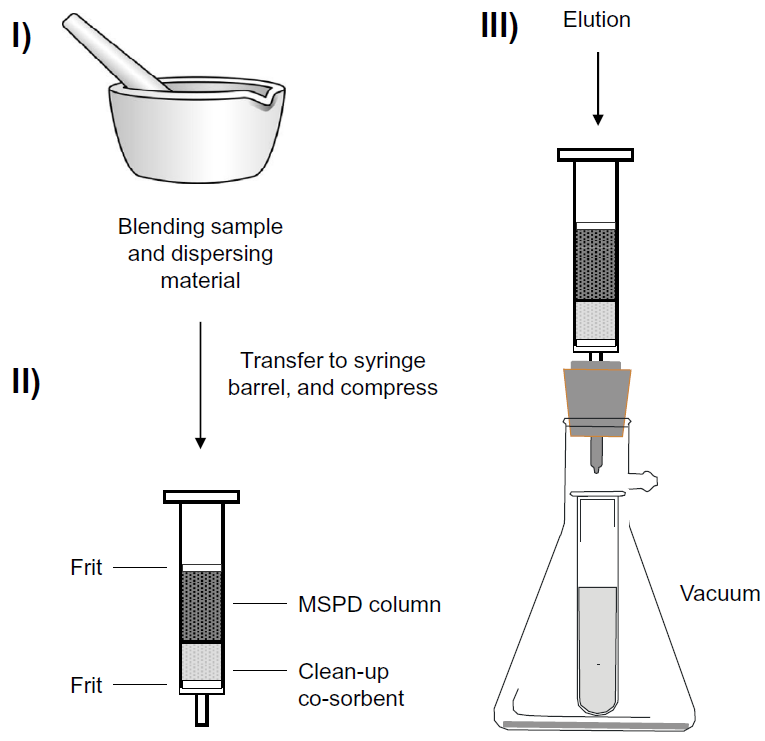
\includegraphics[width=0.8\textwidth]{Images/mspd.PNG}
\caption{M\'etodo MSPD$^{\cite{Capriotti2015}}$.}
\label{mspd}
\end{figure}

\subsection{Factores a considerar en la extracci\'on MSPD}

\noindent
\justify

Hay varios factores a considerar en la extracci\'on MSPD, que incluye:

\begin{enumerate}
	\item \textit{Efecto del tama\~no de part\'icula media:} tama\~nos de part\'icula peque\~nos (entre $3$ - $10 \, \mu m$) requiere de grandes tiempos de eluci\'on y altos gradientes de presi\'on para obtener un flujo adecuado. 
	\item \textit{Agente dispersante:} el uso de silicatos infravalorados, como la arena de r\'io, para la maceraci\'on de muestras presenta resultados diferentes a los reportados con agentes dispersantes como el $C_{18}$ o el $C_8$. A pesar de que el mismo principio de disrupci\'on de la matriz se conserva, debido a la abrasi\'on, es probable que se de una interacci\'on qu\'imica no deseada entre silicatos infravalorados y algunos de los flavonoides del extracto.
	\item \textit{Relaci\'on m\'asica:} la mejor relaci\'on m\'asica reportada en la literatura frecuenta ser una relaci\'on 1 a 4 $^{\cite{barker2007}}$, aunque puede variar de una aplicaci\'on a otra. 
	\item \textit{Solvente:} el vertimiento del solvente en la columna MSPD tiene el fin de aislar analitos espec\'ificos o familias de compuestos. El tipo de solvente, y la polaridad de este, define la composici\'on final del extracto. Existen estudios en donde se ha demostrado un incremento en el rendimiento extractivo al emplear solventes a temperaturas superiores a la temperatura ambiente e inferiores a los $60 \left[ \degree C \right]^{\cite{Vieira2019}}$. 
\end{enumerate}

\subsection{Extracci\'on en fase s\'olida}

\noindent
\justify

El m\'etodo MSPD presenta diferencias claras respecto a la extracci\'on fase s\'olida cl\'asica (SPE, por sus siglas en ingl\'es); entre ellas$^{\cite{barker2007}}$:
\begin{enumerate}
	\item Al emplear el m\'etodo MSPD, se consigue una disrupci\'on completa de la muestra en part\'iculas de reducido tama\~no, incrementando el \'area de extracci\'on. En SPE, la disrupci\'on de la muestra se considera un paso \textit{adicional}, donde muchos de los compuestos se descartan al procesar la muestra para la columna SPE. 
	\item En SPE, la muestra es usualmente absorbida en la parte superior de la columna y no a trav\'es de ella, como en el m\'etodo MSPD.
	\item La interacci\'on f\'isica y qu\'imica de los compuestos del sistema son mayores en el m\'etodo MSPD y diferentes, en diversos sentidos, de aquellos apreciados en el SPE cl\'asico, incluyendo otras formas de cromatograf\'ia l\'iquida.
\end{enumerate}

\newpage

\subsection{Prototipo a escala}

\noindent
\justify

Se han desarrollado estudios experimentales sobre un prototipo a escala de una planta de extracci\'on con capacidad productiva de $1 [kg / bache]$, tres baches al d\'ia. El flujo de trabajo se puede apreciar en la Figura \ref{cadena}.

\begin{figure}[h!]
	\centering
	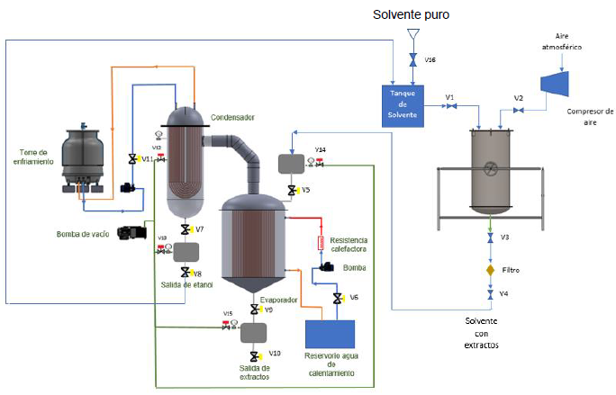
\includegraphics[width=1.1\textwidth]{Images/planta.PNG}
	\caption{Prototipo desarrollado$^{\cite{Proyecto, Patente2018}}$.}
	\label{cadena}
\end{figure}

La invenci\'on desarrollada consiste de:
\begin{itemize}
	\item Molino de bolas dise\~nado como recipiente a presi\'on.
	\item Unidad compresora de aire.
	\item Evaporador.
	\item Condensador.
	\item Sistema de calentamiento de agua por resistencia el\'ectrica.
	\item Torre de enfriamiento.
\end{itemize}




\subsection{Din\'amica de Fluidos Computacional} \label{DFC}

\noindent
\justify

La \textit{Din\'amica de Fluidos Computacional} (CFD, por sus siglas en ingl\'es) es una herramienta computacional ampliamente usada en ingenier\'ia para el desarrollo de simulaciones num\'ericas que involucren fluidos. Emplea como m\'etodo base el m\'etodo de vol\'umenes finitos (FVM). Este m\'etodo num\'erico transforma las ecuaciones diferenciales parciales, que representan las leyes conservativas, en ecuaciones algebraicas discretas sobre vol\'umenes finitos. 

\noindent
\justify

Inicia con la discretizaci\'on del dominio en elementos no superpuestos. Las ecuaciones diferenciales son discretizadas (transformadas) en ecuaciones algebraicas al integrarlas sobre cada dominio de los elementos. El sistema de ecuaciones algebraicas es luego resulto para calcular los valores de las variables dependientes de cada elemento. Algunos de los t\'etminos en la ecuaci\'on de conservaci\'on se convierten en flujos que se eval\'uan sobre las caras de los elementos. Es `sencillo' evaluar condiciones de frontera, tanto de tipo \textit{Dirichlet} como \textit{Neumann}, de manera no invasiva, dado que las variables desconocidas se eval\'uan en los centroides de los elementos, no en las caras de los mismos, como se aprecia en la Figura \ref{elemento}. Estas caracter\'istias lo hacen adecuado para que la simulaci\'on presente una variedad de aplicaciones que involucran: flujo de fluidos y transferencia de calor y masa.

\noindent
\justify

B\'asicamente, con este m\'etodo num\'erico se busca resolver los siguientes grupos de ecuaciones:

\begin{itemize}
	\item Ecuaci\'on de continuidad:
	\begin{equation*}
		\frac{\partial u}{\partial x} + \frac{\partial v}{\partial y} = 0
	\end{equation*}
	\item Ecuaciones de momento:
	\begin{equation*}
			\frac{\partial u}{\partial t} + u \frac{\partial u}{\partial x} + v \frac{\partial u}{\partial y} = - \frac{1}{\rho} \frac{\partial p}{\partial x} + \frac{\mu}{\rho} \left( \frac{\partial ^2 u}{\partial x ^2} + \frac{\partial ^2 u}{\partial y ^2} \right)
	\end{equation*}
	\begin{equation*}
			\frac{\partial v}{\partial t} + u \frac{\partial v}{\partial x} + v \frac{\partial v}{\partial y} = - \frac{1}{\rho} \frac{\partial p}{\partial y} + \frac{\mu}{\rho} \left( \frac{\partial ^2 v}{\partial x ^2} + \frac{\partial ^2 v}{\partial y ^2} \right)
	\end{equation*}
\end{itemize}

\noindent
\justify

De estas ecuaciones, los componentes desconocidos suelen ser la presi\'on y velocidad. Se requieren condiciones iniciales y de frontera para definir el problema.No hay una ecuaci\'on espec\'ifica para definir la presi\'on. Para flujos incompresibles, la presi\'on es el campo que hace que la velocidad logre cumplir la ley de la conservaci\'on de la masa$^{\cite{Abou-Hweij2020}}$.

\noindent
\justify

Los m\'etodos num\'ericos se enfocan tanto en el proceso de discretizaci\'on como en el m\'etodo de soluci\'on del grupo de ecuaciones algebraicas obtenidas. La \textbf{precisi\'on} de una soluci\'on num\'erica est\'a arraigada al m\'etodo de discretizaci\'on$^{\cite{Bao2021}}$.

\begin{figure}[h!]
	\centering
	\begin{tikzpicture}
 		\draw (0,0) rectangle (12,7);
 		\foreach \x in {1,...,4}{
			\draw (\x*3,0) -- (\x*3,7); 		
 		}
 		\foreach \y in {1,...,3}{
			\draw (0, \y*2.33) -- (12,\y*2.33); 		
 		}	
 		\draw[pattern=north west lines, pattern color=blue!55!red] (3,2.33) rectangle (6,4.66);	
 		\draw[fill=cyan] (4.5,3.5) circle (0.2cm);
 		\draw[-triangle 90, fill=black] (7.5,3.5) -- (4.7,3.5);
 		\node[align=right] at (7.5,3.5) {Centroide del \\ elemento};
 		\node[color=black] at (4.5,3) {Elemento};
 		\draw (9,4.66) circle (0.1cm);
 		\draw[-triangle 90, fill=black] (10.5,5.3) -- (9.15,4.8);
 		\node[align=right] at (10.5,5.5) {(V\'ertice)};
	\end{tikzpicture}
	\caption{Discretizaci\'on del dominio (malla cartesiana).}
	\label{elemento}
\end{figure}

\newpage

\noindent
\justify

Existen dos tipos de mallas para el an\'alisis mediante CFD, como se aprecia en la Figura \ref{mallas}.

\begin{figure}[h!]
	\centering
	\begin{subfigure}[b]{0.48\textwidth}
		\centering
		\begin{adjustbox}{max width = \textwidth}
		\begin{tikzpicture}
			\begin{axis}[grid=both,view={70}{40},colormap/viridis]
  				\addplot3+[surf,mesh/rows=11,mesh/ordering=colwise,no marks] file {malla.txt};
			\end{axis}
		\end{tikzpicture}
		\end{adjustbox}
		\caption{Malla estructurada.}
	\end{subfigure}
	\hfill
	\begin{subfigure}[b]{0.5\textwidth}
		\centering
		\begin{adjustbox}{max width = \textwidth}
		\begin{tikzpicture}
			\foreach \i [evaluate={\ii=int(\i-1);}] in {0,...,6}{
  			\foreach \j [evaluate={\jj=int(\j-1);}] in {0,...,6}{
    			\coordinate [shift={(\j,\i)}] (n-\i-\j) at (rand*270:1/2+rnd/8);
				\ifnum\i>0
  					\draw [help lines] (n-\i-\j) -- (n-\ii-\j);
				\fi
				\ifnum\j>0
  					\draw [help lines] (n-\i-\j) -- (n-\i-\jj);
				\fi
			}}
		\end{tikzpicture}
		\end{adjustbox}
	\caption{Malla no estructurada.}
	\end{subfigure}
	\caption{Tipos de mallas.}
	\label{mallas}
\end{figure}

\noindent
\justify

La conversi\'on de las ecuaciones diferenciales parciales requieren la discretizaci\'on del dominio de estudio; que, a su vez, depende de la dimensionalidad del problema.

\subsubsection{Solucionadores}

\noindent
\justify

Existen diferentes m\'etodos de soluci\'on de sistemas de ecuaciones algebraicas que pueden ser: \textit{exactos} o \textit{iterativos}. Los solucionadores que emplean m\'etodos exactos no suelen usarse en simulaciones num\'ericas debido al alto costo computacional. B\'asicamente tratan de resolver el sistema matricial $A \phi = B \rightarrow \phi = A^{-1} B$. 

\noindent
\justify

Los m\'etodos iterativos suelen basarse en la l\'ogica de \textit{suposici\'on} y \textit{corroboraci\'on}. El m\'etodo de Gauss - Seidel$^{\cite{Bai2021}}$, por ejemplo, inicia suponiendo el valor de una variable, corrobor\'andola con el c\'alculo de las dem\'as; en caso de no coincidir, su supone el resultado final de la variable supuesta, donde se vuelve a corroborar hasta que el supuesto y la corroboraci\'on coincidan o hasta que el margen de error sea tolerable.

\subsubsection{Metodolog\'ias de verificaci\'on y validaci\'on} \label{verified}

\noindent
\justify

Tienen por objetivo garantizar el menor \textit{error computacional} posible. Entre ellas se destacan:

\begin{itemize}
	\item \textit{Simple}: estudio de la evoluci\'on global o local de una variable debido al refinamiento de malla, como se aprecia en la Figura \ref{valsimple}.
	\begin{figure}[h!]
	\centering
	\begin{tikzpicture}
		\begin{axis}[
			domain = 0:1000,
			grid = both, minor tick num=2,
			title = \textbf{Validaci\'on por refinamiento de malla},
			xlabel = N\'umero de nodos,
			ylabel = Valor,
			legend pos = outer north east,
			restrict y to domain* = 0:100,
			width=10cm, height=8cm
		]
		\addplot[blue, line width=2pt] {\val};
		\addplot[
        scatter,scatter src=explicit symbolic,
        scatter/classes={
            a={mark=o,black},
            b={mark=triangle*,red},
            c={mark=o,draw=black,fill=black}
        }
    ]
    table[x=x,y=y,meta=label]{
        x	y	label
		10	30	a
		15	32	a
		30	43	a
		60	55	a
		100	70	a
		300	80	a
		600	92	a
		800	95	a
		1000	96	a

    };
		\legend{Te\'orico, Num\'erico};
		\end{axis}
	\end{tikzpicture}
	\caption{M\'etodo de validaci\'on simple.}
	\label{valsimple}
	\end{figure}
	\item \textit{Detallada}: se basa en la extrapolaci\'on generalizada de Richardson y en el \'indice de convergencia de malla (GCI).
	\item \textit{Experimentaci\'on}: se validan los resultados con estudios experimentales.
\end{itemize}

\subsubsection{An\'alisis bidimensional - 2D} \label{CFD2D}

\noindent
\justify

Para an\'alisis bidimensional, se busca resolver la Ecuaci\'on \ref{2DCFD}.

\begin{equation}
\underbrace{\rho \frac{\partial \phi}{\partial t}}_{\text{transitorio}} + \underbrace{\rho u \frac{\partial \phi}{\partial x} + \rho v \frac{\partial \phi}{\partial y}}_{\text{convectivo}} = \underbrace{ \frac{\partial}{\partial x} \left( \Gamma \frac{\partial \phi}{\partial x} \right) + \frac{\partial}{\partial y} \left( \Gamma \frac{\partial \phi}{\partial y} \right)}_{\text{difusivo}} + \underbrace{S_{\phi}}_{\text{fuente}}
\label{2DCFD}
\end{equation}

\noindent
\justify

La discretizaci\'on del dominio se realiza acorde a la Figura \ref{dis2D}.

\begin{figure}[h!]
\centering
\begin{tikzpicture}
\draw (0,0) rectangle (6,6);
\newcounter{contx} %counter
\setcounter{contx}{0}
\newcounter{conty} %counter
\setcounter{conty}{0}
\foreach \x in {0,1.5,3,4.5}
    \foreach \y in {0,1.5,3,4.5}
      {
        \draw (\x,\y) rectangle (\x + 1.5, \y + 1.5);
        \draw[fill=black] (\x + 0.75, \y + 0.75) circle (0.5mm);
        \stepcounter{conty}
        \ifnum \value{contx}<3
        	\draw[red, -triangle 90, fill=red] (\x+1.3, \y + 0.75) -- (\x+1.7, \y + 0.75);
        \fi
        \ifnum \value{conty}=4
        	\setcounter{conty}{0}
        	\stepcounter{contx}
        \else
        	\draw[blue, -triangle 90, fill=blue] (\x+0.75, \y + 1.3) -- (\x+0.75, \y + 1.7);
        \fi
      }

\foreach \x in {0,1.5,3,4.5}
	{
		\draw[fill=black] (\x + 0.75, 0) circle (0.5mm);
		\draw[fill=black] (\x + 0.75, 6) circle (0.5mm);
	}

\foreach \y in {0,1.5,3,4.5}
	{
		\draw[fill=black] (0, \y + 0.75) circle (0.5mm);
		\draw[fill=black] (6, \y + 0.75) circle (0.5mm);
	}

\node at (2.5,2.5) {P};
\node at (4,2.5) {E};
\node at (2.5,4) {N};
\node at (2.5,1) {S};
\node at (1,2.5) {W};

\end{tikzpicture}
\caption{Discretizaci\'on dominio bidimensional.}
\label{dis2D}
\end{figure}

\noindent
\justify

Existen diferentes enfoques para el an\'alisis de problemas bidimensionales, entre ellos se encuentran: diferencias centradas, \textit{upwind} e h\'ibrido. El acercamiento por diferencias centradas asume una variaci\'on lineal de $\phi$ entre nodos para una malla uniforme, de modo que:

\begin{equation}
\begin{array}{c}
	a_P \phi _P = a_E \phi _E  + a_W \phi _W + a_N \phi _N + a_S \phi _S + b \\
	a_E = D_e - F_e/2 \\
	a_W = D_w + F_w/2 \\
	a_N = D_n - F_n/2 \\
	a_S = D_s + F_s/2 \\
	a_P = a_E + a_W + a_N + a_S + \rho \frac{\Delta x \Delta y}{\Delta t} + \left(F_e - F_w + F_n - F_s \right) \\
	b = \rho \frac{\Delta x \Delta y}{\Delta t} \phi _P ^0 + S \Delta x \Delta y
\end{array}
\end{equation}

\subsection{M\'etodo de Elementos Discretos}


\noindent
\justify

El m\'etodo de elementos discretos (DEM) es un m\'etodo que modela fuerzas interpart\'icula basadas en par\'ametros de elasticidad y la superposici\'on de part\'iculas no deformadas, que se entiende como la cantidad de deformaci\'on necesaria para que puedan, f\'isicamente, ocupar el espacio en su actual configuraci\'on. Requiere de seis grados de libertad en cuerpos r\'igidos: tres en dos dimensiones y seis en tres dimensiones.

\begin{figure}[h!]
	\centering
	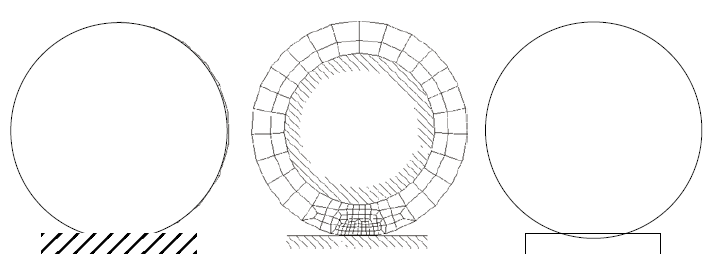
\includegraphics[width=\textwidth]{Images/DEM.PNG}
	\label{dem}
	\caption{Comparaci\'on entre metodolog\'ias de an\'alisis de part\'iculas para una esfera suave deformada en un plano: situaci\'on f\'isica real (izquierda), modelo analizado con el m\'etodo de elementos finitos (centro) y modelo con el m\'etodo de elementos discretos (derecha). Fuente: \v Smilauer 2015$^{\cite{Smilauer2015}}$.}
\end{figure}

\noindent
\justify

El principio de este m\'etodo es el de computar las fuerzas proporcionales a la superposici\'on geom\'etrica de las part\'iculas empleadas. Para part\'iculas esf\'ericas, o circulares, las fuerzas involucradas son de tipo central; a diferencia de otras configuraciones geom\'etricas, debido a que deben caracterizar las fuerzas en la forma `d\'ebil' y `fuerte'. 

\noindent
\justify

Una simulaci\'on que emplea este m\'etodo num\'erico, normalmente se rige bajo los siguientes pasos:

\begin{enumerate}
	\item Detecci\'on de colisi\'on entre part\'iculas.
	\item Creaci\'on de una nueva interacci\'on y determinaci\'on de diferentes propiedades, entre ellas la rigidez.
\end{enumerate}

\noindent
\justify

Para interacciones ya existentes:

\begin{enumerate}
	\item Evaluaci\'on de deformaci\'on.
	\item Computaci\'on del esfuerzo basada en la deformaci\'on.
	\item Aplicaci\'on de fuerzas en la interacci\'on entre part\'iculas.
\end{enumerate}

\subsubsection{Detecci\'on de una colici\'on} \label{detect}

\noindent
\justify

La detecci\'on \textit{exacta} de colisi\'on entre dos part\'iculas requiere de un alto costo computacional. Tomando una pareja de cuerpos $i$ y $j$ y su colisici\'on `exacta' (en el sentido de precisi\'on admisible por la implementaci\'on num\'erica) presentadas en los puntos $P_i$ y $P_j$ la detecci\'on procede en los siguientes dos puntos:

\begin{enumerate}
	\item Detecci\'on de colisi\'on r\'apida usando puntos aproximados $\widetilde{P}_i$ y $\widetilde{P}_j$; siendo estos preconstrucciones en el modo que caracter\'isticas individuales $P_i$ y $P_j$ satisfacen la siguiente condici\'on mostrada en la Ecuaci\'on \ref{cond}.
	\begin{equation}
		\forall x \in R^3 : x \in P_i \rightarrow x \in \widetilde{P}_i
		\label{cond}
	\end{equation}
	De igual manera para $P_j$. El predicado aproximaado se conoce como `volumen l\'imite', siguiendo lo siguiente:
	\begin{equation}
		\left(\widetilde{P}_i \cap \widetilde{P}_j \right) = {\O} \rightarrow \left( P_i \cap P_j \right) = {\O}
		\label{imposible}
	\end{equation}
	\item Al filtrar las colisiones imposibles mediante la Ecuaci\'on \ref{imposible}, algoritmos de detecci\'on de mayor costo computacional pueden ser impementados al filtrar falsas parejas de colisi\'on restantes, como se observa en la Figura \ref{colision}.
	\begin{equation}
		\left(\widetilde{P}_i \cap \widetilde{P}_j \right) \neq {\O} \wedge \left(P_i \cap P_j \right) = {\O}
	\end{equation}
\end{enumerate}

\begin{figure}[h!]
\centering
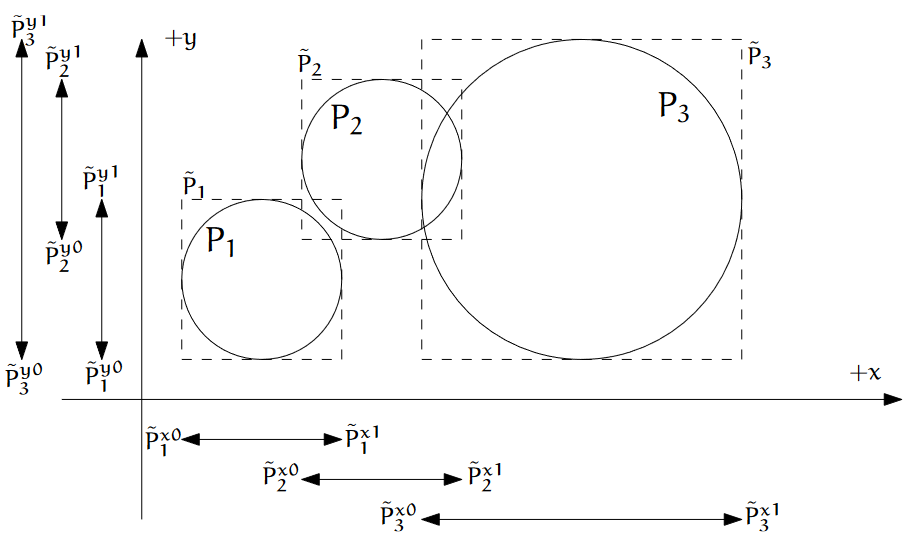
\includegraphics[width=0.9\textwidth]{Images/Colision.PNG}
\caption{Detecci\'on de colisi\'on entre part\'iculas. Fuente: \v Smilauer 2015$^{\cite{Smilauer2015}}$.}
\label{colision}
\end{figure}

\noindent
\justify

Yade$^{\cite{Smilauer2015}}$ emplea un algoritmo conocido como ``\texttt{Aabb}" (\textit{Caja de contorno para alineaci\'on de eje}, por sus siglas en ingl\'es); visualmente, consisten en los rect\'angulos de contorno que rodean cada esfera de la Figura \ref{colision}. Cada caja de contorno es usada como $\widetilde{P}_i$; estando definida cada una por sus esquinas $\varepsilon R^3$ siendo $\widetilde{P}_i ^{x0}$ y $\widetilde{P}_i ^{x1}$ las coordenadas en el eje $x$ de la esfera $P_1$, por ejemplo. 

\noindent
\justify

La presencia de superposici\'on entre part\'iculas entre dos \texttt{Aabb}'s se determina mediante el conjunto de superposici\'on separada de intervalos sobre cada eje. Est\'a representada por la Ecuaci\'on \ref{overlap:dem}.

\begin{equation}
	\left(\widetilde{P}_i \cap \widetilde{P}_j \right) \neq {\O} \Longleftrightarrow \bigwedge_{w \epsilon \{x,y,z \}} \left[\left(\left(\widetilde{P}_i ^{w0}, \widetilde{P}_i ^{w1} \right) \cap \left(\widetilde{P}_j ^{w0}, \widetilde{P}_j ^{w1} \right) \right) \neq {\O} \right] 
	\label{overlap:dem}
\end{equation}

\begin{center}
	\section{M\'etodo CFD-DEM}
\end{center}

\noindent
\justify

En el acoplamiento cl\'asico entre CFD-DEM, el flujo se resuelve a trav\'e del m\'etodo CFD basado en malla, mientras que la fase s\'olida es modelada mediante DEM para cada part\'icula sujeta a trav\'es de fuerzas hidrodin\'amicas, fuerzas de cuerpo (como la gravedad) y a trav\'es de fuerzas de contacto, actualizando valores de velocidad y posici\'on conforme a la segunda ley de Newton (Hoomans \textit{et al.}, 1996; Tsuji \textit{et al.}, 1993; Xu y Yu, 1997). En principio, todos los m\'etodos CFD pueden acoplarse con DEM; lo que ha dado origen a diferentes m\'etodos discretos y continuos, tal como el m\'etodo de Lattice Boltzmann (LBM), Hidrodin\'amica de Part\'iculas Suaves (SPH), m\'etodos de Diferencias Finitas y Vol\'umenes Finitos (FVM).

\noindent
\justify

Gran parte de las simulaciones reportadas en la literatura comprenden modelos 2D o sistemas prototipados de peque\~na escala. En busca de acelerar los tiempos de simulaci\'on e incrementar la eficiencia computacional, se han desarrollado t\'ecnicas de computaci\'on paralela; donde gran parte de los esfuerzos han sido enfocados en la paralelizaci\'on del DEM. Muchos algoritmos se han propuesto para lograr este hecho, como la t\'ecnica de espejo de dominio (Damana, \textit{et al.}, 2006; Washington y Meegoda, 2003), el m\'etodo de subconjunto de part\'iculas (Kafui \textit{et al.}, 2011) y m\'etodos de descomposici\'on de dominios (Amritkar \textit{et al.}, 2014; Tsuji \textit{et al.}, 2008). El uso de estos algoritmos depende de la arquitectura del hardware. La paralelizaci\'on sobre memoria compartida del sistema se alcanza, normalmente, empleando \textit{OpenMP} (``Open Multi-Processing", por sus siglas en ingl\'es), mientras que el MPI (Interfaz de Paso de Mensajes) se emplea en sistemas de memoria distirbuida (Rabenseifner \textit{et al.}, 2009). Por ejemplo, Tsuji \textit{et al.} (2008) paralelizaron una simulaci\'on en CFD-DEM usando MPI para el intercambio de informaci\'on entre 16 CPUs, reportando el comportamiento fluidodin\'amico de 4.5 millones de part\'iculas en un medio gaseoso; empleando el m\'etodo unidimensional de descomposici\'on de dominio.

\subsection{Fase del solvente}

\noindent
\justify

En un modelo CFD-DEM, la fase del fluido se resuleve en el nivel computacional en cada elemento de la malla (ver Figura \ref{elemento}) empleando un marco de referencia Euleriano mientras que el movimiento de la part\'icula se sigue a trav\'es de un marco de referencia Lagrangiano. Para lograr el acoplamiento de fase, es necesario interpolar las propiedades de las part\'iculas a los centroides de los elementod CFD y las propiedades del fluido a la posici\'on de cada part\'icula. Como se muestra en la Figura \ref{particle}, se crean dos mallas alineadas de b\'usqueda: la malla de b\'usqueda de part\'iculas (amarilla) y la malla de b\'usqueda de fluido (azul). 

\begin{figure}[h!]
	\centering
	\begin{subfigure}[b]{0.3\textwidth}
		\centering
		\begin{adjustbox}{max width = \textwidth}
		\begin{tikzpicture}
		%---Interno---
	%1 - (-1.2, -0.4)
	\draw[white, fill=blue!30!gray!30!white] (-1.5, -1.5) -- (0,-1.6) -- (-1.2, -0.4) -- cycle;
	\draw[white, fill=blue!30!gray!30!white] (-2.2, 1) -- (-1.5,-1.5) -- (-1.2, -0.4) -- cycle;
	\draw[white, fill=blue!30!gray!30!white] (-2.2, 1) -- (-0.5, 1.55) -- (-1.2, -0.4) -- cycle;
	%2 - (0.7, -0.5)
	\draw[white, fill=blue!30!gray!30!white] (-1.2, -0.4) -- (0,-1.6) -- (0.7, -0.5) -- cycle;
	\draw[white, fill=blue!30!gray!30!white] (0.8,-2) -- (0,-1.6) -- (0.7, -0.5) -- cycle;
	\draw[white, fill=blue!30!gray!30!white] (1.8,-1.5) -- (0.8,-2) -- (0.7, -0.5) -- cycle;
	\draw[white, fill=blue!30!gray!30!white] (1.8,-1.5) -- (1.7,0) -- (0.7, -0.5) -- cycle;
	%3 - (0.5,0.8)
	\draw[white, fill=blue!30!gray!30!white] (1.7,0) -- (1.8,1.5) -- (0.5, 0.8) -- cycle;
	\draw[white, fill=blue!30!gray!30!white] (1.7,0) -- (0.7, -0.5) -- (0.5, 0.8) -- cycle;
	\draw[white, fill=blue!30!gray!30!white] (1,2.2) -- (1.8,1.5) -- (0.5, 0.8) -- cycle;
	\draw[white, fill=blue!30!gray!30!white] (-0.5,1.55) -- (1,2.2) -- (0.5, 0.8) -- cycle;
	\draw[white, fill=blue!30!gray!30!white] (-1.2,-0.4) -- (0.7,-0.5) -- (0.5, 0.8) -- cycle;
	\draw[white, fill=blue!30!gray!30!white] (-1.2,-0.4) -- (-0.5,1.55) -- (0.5, 0.8) -- cycle;
	
	%malla
	\draw[step=0.5, dashed, yellow!90!black] (-2.2, -2) grid (1.9,2.2);
	
	%Partículas
	\draw[black!50, fill=red!50] (0,0) circle (2mm);
	\draw[black!50, fill=yellow!50] (0.6,-0.6) circle (2mm);
	\draw[black!50, fill=yellow!50] (-1.1,-0.3) circle (2mm);
	\draw[black!50, fill=yellow!50] (0.5,0.9) circle (2mm);
	\draw[black!50, fill=yellow!50] (-0.5,0.5) circle (2mm);
	\draw[black!50, fill=yellow!50] (1.2,0.2) circle (2mm);
	\draw[black!50, fill=yellow!50] (-0.5,-0.8) circle (2mm);
	\draw[black!50, fill=yellow!50] (0.2,-1) circle (2mm);
	
	\draw[black!50, fill=blue!70] (1.7,-1.3) circle (2mm);
	\draw[black!50, fill=blue!70] (-1.4,-1.4) circle (2mm);
	\draw[black!50, fill=blue!70] (-1,0.4) circle (2mm);
	\draw[black!50, fill=blue!70] (-1.7, 0.5) circle (2mm);
	\draw[black!50, fill=blue!70] (-1.3,1.45) circle (2mm);
	\draw[black!50, fill=blue!70] (1.2, 1.1) circle (2mm);
	\draw[black!50, fill=blue!70] (0.5,1.4) circle (2mm);
	\draw[black!50, fill=blue!70] (1.3,1.8) circle (2mm);
	
	%Carcasa
	\draw[black!60] (-2.2, 1) -- (-0.5, 1.55) -- (1, 2.2) -- (1.8, 1.5) -- (1.7, 0) -- (1.8, -1.5) -- (0.8, -2) -- (0, -1.6) -- (-1.5, -1.5) -- cycle;
	 
	 %Círculo rojo
	\draw[red!60!black, dashed] (0,0) circle (1.5 cm);
		\end{tikzpicture}
		\end{adjustbox}
		\caption{B\'usqueda de part\'iculas vecinas y c\'alculo de la fracci\'on de vac\'io de una part\'icula dada.}
	\end{subfigure}
	\hfill
	\begin{subfigure}[b]{0.3\textwidth}
		\centering
		\begin{adjustbox}{max width = \textwidth}
		\begin{tikzpicture}
		%---Interno---
	%1 - (-1.2, -0.4)
	\draw[white, fill=blue!30!gray!30!white] (-1.5, -1.5) -- (0,-1.6) -- (-1.2, -0.4) -- cycle;
	\draw[white, fill=blue!30!gray!30!white] (-2.2, 1) -- (-1.5,-1.5) -- (-1.2, -0.4) -- cycle;
	\draw[white, fill=blue!30!gray!30!white] (-2.2, 1) -- (-0.5, 1.55) -- (-1.2, -0.4) -- cycle;
	%2 - (0.7, -0.5)
	\draw[white, fill=blue!30!gray!30!white] (-1.2, -0.4) -- (0,-1.6) -- (0.7, -0.5) -- cycle;
	\draw[white, fill=blue!30!gray!30!white] (0.8,-2) -- (0,-1.6) -- (0.7, -0.5) -- cycle;
	\draw[white, fill=blue!30!gray!30!white] (1.8,-1.5) -- (0.8,-2) -- (0.7, -0.5) -- cycle;
	\draw[white, fill=blue!30!gray!30!white] (1.8,-1.5) -- (1.7,0) -- (0.7, -0.5) -- cycle;
	%3 - (0.5,0.8)
	\draw[white, fill=blue!30!gray!30!white] (1.7,0) -- (1.8,1.5) -- (0.5, 0.8) -- cycle;
	\draw[white, fill=blue!30!gray!30!white] (1.7,0) -- (0.7, -0.5) -- (0.5, 0.8) -- cycle;
	\draw[white, fill=blue!30!gray!30!white] (1,2.2) -- (1.8,1.5) -- (0.5, 0.8) -- cycle;
	\draw[white, fill=blue!30!gray!30!white] (-0.5,1.55) -- (1,2.2) -- (0.5, 0.8) -- cycle;
	\draw[white, fill=blue!30!gray!30!white] (-1.2,-0.4) -- (-0.5,1.55) -- (0.5, 0.8) -- cycle;
	\draw[white, fill=red!30!yellow!30!white] (-1.2,-0.4) -- (0.7,-0.5) -- (0.5, 0.8) -- cycle;
	
	%malla
	\draw[step=1, dashed, blue!90!black] (-2.2, -2) grid (1.9,2.2);
	
	%Partículas
	\draw[black!50, fill=red!50] (0,0) circle (2mm);
	
	%Carcasa
	\draw[black!60] (-2.2, 1) -- (-0.5, 1.55) -- (1, 2.2) -- (1.8, 1.5) -- (1.7, 0) -- (1.8, -1.5) -- (0.8, -2) -- (0, -1.6) -- (-1.5, -1.5) -- cycle;
	 
		\end{tikzpicture}
		\end{adjustbox}
	\caption{Mapeo de una part\'icula dada dentro del fluido para interpolar sus propiedades en ese punto.}
	\end{subfigure}
	\hfill
	\begin{subfigure}[b]{0.3\textwidth}
		\centering
		\begin{adjustbox}{max width = \textwidth}
		\begin{tikzpicture}
		%---Interno---
	%1 - (-1.2, -0.4)
	\draw[white, fill=blue!30!gray!30!white] (-1.5, -1.5) -- (0,-1.6) -- (-1.2, -0.4) -- cycle;
	\draw[white, fill=blue!30!gray!30!white] (-2.2, 1) -- (-1.5,-1.5) -- (-1.2, -0.4) -- cycle;
	\draw[white, fill=blue!30!gray!30!white] (-2.2, 1) -- (-0.5, 1.55) -- (-1.2, -0.4) -- cycle;
	%2 - (0.7, -0.5)
	\draw[white, fill=blue!30!gray!30!white] (-1.2, -0.4) -- (0,-1.6) -- (0.7, -0.5) -- cycle;
	\draw[white, fill=blue!30!gray!30!white] (0.8,-2) -- (0,-1.6) -- (0.7, -0.5) -- cycle;
	\draw[white, fill=blue!30!gray!30!white] (1.8,-1.5) -- (0.8,-2) -- (0.7, -0.5) -- cycle;
	\draw[white, fill=blue!30!gray!30!white] (1.8,-1.5) -- (1.7,0) -- (0.7, -0.5) -- cycle;
	%3 - (0.5,0.8)
	\draw[white, fill=blue!30!gray!30!white] (1.7,0) -- (1.8,1.5) -- (0.5, 0.8) -- cycle;
	\draw[white, fill=blue!30!gray!30!white] (1.7,0) -- (0.7, -0.5) -- (0.5, 0.8) -- cycle;
	\draw[white, fill=blue!30!gray!30!white] (1,2.2) -- (1.8,1.5) -- (0.5, 0.8) -- cycle;
	\draw[white, fill=blue!30!gray!30!white] (-0.5,1.55) -- (1,2.2) -- (0.5, 0.8) -- cycle;
	\draw[white, fill=red!95!yellow!60!white] (-1.2,-0.4) -- (0.7,-0.5) -- (0.5, 0.8) -- cycle;
	\draw[white, fill=blue!30!gray!30!white] (-1.2,-0.4) -- (-0.5,1.55) -- (0.5, 0.8) -- cycle;
	
	%malla
	\draw[step=0.5, dashed, yellow!90!black] (-2.2, -2) grid (1.9,2.2);
	
	%Partículas
	\draw[black!50, fill=red!50] (0,0) circle (2mm);
	\draw[black!50, fill=yellow!50] (0.6,-0.6) circle (2mm);
	\draw[black!50, fill=yellow!50] (-1.1,-0.3) circle (2mm);
	\draw[black!50, fill=yellow!50] (0.5,0.9) circle (2mm);
	\draw[black!50, fill=yellow!50] (-0.5,0.5) circle (2mm);
	\draw[black!50, fill=yellow!50] (1.2,0.2) circle (2mm);
	\draw[black!50, fill=yellow!50] (-0.5,-0.8) circle (2mm);
	\draw[black!50, fill=yellow!50] (0.2,-1) circle (2mm);
	
	\draw[black!50, fill=blue!70] (1.7,-1.3) circle (2mm);
	\draw[black!50, fill=blue!70] (-1.4,-1.4) circle (2mm);
	\draw[black!50, fill=blue!70] (-1,0.4) circle (2mm);
	\draw[black!50, fill=blue!70] (-1.7, 0.5) circle (2mm);
	\draw[black!50, fill=blue!70] (-1.3,1.45) circle (2mm);
	\draw[black!50, fill=blue!70] (1.2, 1.1) circle (2mm);
	\draw[black!50, fill=blue!70] (0.5,1.4) circle (2mm);
	\draw[black!50, fill=blue!70] (1.3,1.8) circle (2mm);
	
	%Carcasa
	\draw[black!60] (-2.2, 1) -- (-0.5, 1.55) -- (1, 2.2) -- (1.8, 1.5) -- (1.7, 0) -- (1.8, -1.5) -- (0.8, -2) -- (0, -1.6) -- (-1.5, -1.5) -- cycle;
	
	\draw[yellow, fill=red!40!blue, fill opacity=0.2] (-1,-1) rectangle (1,1);
		\end{tikzpicture}
		\end{adjustbox}
	\caption{Mapeo del elemento de malla CFD para el c\'alculo de t\'erminos fuente en el elemento de inter\'es.}
	\end{subfigure}
	\caption{Esquema de la aproximaci\'on por malla dual para la b\'usqueda de part\'iculas vecinas en un fluido.}
	\label{particle}
\end{figure}

\noindent
\justify

Los pasos clave con los que se basan las mallas de b\'usqueda son: detecci\'on de colisi\'on de part\'iculas (descrito en la secci\'on \ref{detect}), geometr\'ia de los elementos de malla CFD (detallado en la secci\'on \ref{CFD2D}) y el c\'alculo de fuerzas de fluido, entre otras.

\noindent
\justify

Para el c\'alculo de las fuerzas ejercidas por el fluido, se requiere conocer las propiedades del fluido en la posici\'on de la part\'icula; incluyendo el gradiente de presi\'on, la velocidad del flujo y el gradiente de velocidades (para fluidos gaseosos). Normalmente, las propiedades del fluido se `almacenan' en el centroide de los elementos de malla durante c\'alculos mediante FVM, como se muestra en la Ecuaci\'on \ref{properties}.

\begin{equation}
\phi _p = \phi _{el} + \nabla \phi _{el} \cdot r_{pc}
\label{properties}
\end{equation}

\noindent
\justify

D\'onde: $\phi _p$ y $\phi _{el}$ son las propiedades del fluido en la posici\'on de la part\'icula y el centroide del elemento, respectivamente; y $r_{pc}$ es el vector distancia que va desde el centro del elemento hasta la posici\'on de la part\'icula. 

\begin{center}
	\section{Sedimentaci\'on}
\end{center}

\noindent
\justify

La sedimentaci\'on es uno de los procesos m\'as antiguos en el tratamiento del agua y consiste en la deposici\'on de materiales s\'olidos de mayor peso que el agua.

\noindent
\justify

Existen cinco tipos de sedimentaci\'on que se clasifican de acuerdo a  la clase de part\'icuas, caracter\'isticas superficiales y concentraci\'on de las mismas:

\begin{itemize}
	\item Sedimentaci\'on \textit{discreta:} las part\'iculas no tienden a aglomerarse, mantienen su tama\~no e individualidad. Son generalmente de textura arenosa.
	\item Sedimen \textit{floculenta}: las part\'iculas floculan y tienden a agruparse durante el proceso.
	\item Sedimentaci\'on \textit{m\'asica}: la concentraci\'on de part\'iculas es tan grande que colisionan entre s\'i, sedimentando como una masa.
	\item Sedimentaci\'on por \textit{compresi\'on}: la concentraci\'on de part\'iculas es tan grande que cada una reposa sobre la otra, present\'andose una especie de soporte entre cada una de ellas; el peso de las part\'iculas superiores tiende a compactar a las inferiores.
	\item Sedimentaci\'on de \textit{alta tasa}: es una variaci\'on de la sedimentaci\'on discreta, en la que se insertan placas paralelas con el fin de aumentar la eficiencia de remoci\'on de part\'iculas.
\end{itemize}

\noindent
\justify

La \textit{sedimentaci\'on} realiza la separaci\'on de los s\'olidos m\'as densos que el agua y la \textit{filtraci\'on} separa aquellos que tienen una densidad muy cercana a la del fluido.

\subsection{Sedimentaci\'on con coagulantes}

\noindent
\justify

Se efect\'ua la decantaci\'on de part\'iculas en las c\'amaras de floculaci\'on; el tama\~no y densidad de las part\'iculas y viscosidad del agua desempae\~nar\'an un papel importante en el dimensionamiento de los sedimentadores. Las unidades podr\'an ser circulares o de flujo radial, cuadradas y rectangulares. Si los tanques sedimentadores se dise\~nan en dos o m\'as pisos, podr\'an ser de flujos independientes o de flujo \textit{zig-zag}, de manera que el flujo recorra todos los pisos de la unidad.

\subsection{Sedimentadores de \textit{placas paralelas}}

\noindent
\justify

Se trata de un tipo de sedimentador desarrollado por Hazen A, en 1904, quien expuso el siguiente principio: ``como la acci\'on de un tanque sedimentador depende de su \'area, y no de su profundidad, una subdivisi\'on horizontal producir\'ia una superficie doble para reunir sedimentos en lugar de una sencilla y duplicar\'ia la cantidad de trabajo". 

\noindent
\justify

La diferencia de los sedimentadores de tasa normal y los de alta tasa son:

\begin{itemize}
	\item El fondo del decantador no es horizontal sino inclinado.
	\item La profundidad del decantador es baja, de forma que hay que construir un n\'umero considerable de celdas superpuestas para poder tratar los vol\'umenes de agua.
	\item El flujo \textbf{debe ser laminar}, con n\'umero de Reynolds entre $80$ y $250$.
\end{itemize}

\begin{figure}[h!]
	\centering
	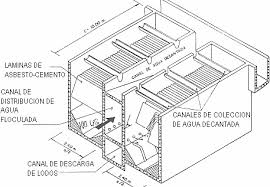
\includegraphics[width=0.7\textwidth]{Images/Sedimentacion/placas.jpg}
	\caption{Sedimentador de placas paralelas.}
	\label{placas}
\end{figure}

\noindent
\justify

Las placas presentan una inclinaci\'on, donde el agua ascendente deposita sobre ellas el material que trae en suspensi\'on. Los lodos resbalan pendiente abajo, y pueden ser recolectados en una tolva en la parte inferior de la estructura.

\begin{equation}
	V_s = \frac{V_0 S}{\sin \theta + \frac{L}{e} \cos \theta}
	\label{CargaSuperficial}
\end{equation}

\noindent
\justify

La Ecuaci\'on \ref{CargaSuperficial}, para un determinado posicionamiento de las placas, permite determinar la velocidad requerida para conseguir una velocidad cr\'itica. Es crucial mantener el n\'umero de Reynolds bajo para evitar que la turbulencia levante los lodos de la cara de las placas donde se est\'a sedimentando.

\subsection{Turbiedad}

\noindent
\justify

La turbidez es la expresi\'on de la propiedad \'optica de la muestra que causa que los rayos de la luz sean dispersados y absorbidos en lugar de ser transmitidos en l\'inea recta a trav\'es de la muestra.

\noindent
\justify

La turbiedad en el agua puede ser causada por la presencia de part\'iculas suspendidas y disueltas de gases, l\'iquidos y s\'olidos tanto org\'anicos como inorg\'anicos.

\noindent
\justify

La eliminaci\'on de la turbiedad se lleva a cabo mediante procesos de coagulaci\'on, asentamiento y filtraci\'on.


\begin{center}
	\section{Metodolog\'ia}
\end{center}

\noindent
\justify

En la Figura \ref{metodologia} se muestra la metodolog\'ia empleada para el dise\~no del sistema de eluci\'on y filtrado de la planta de extracci\'on.

% Define block styles: decision, block, line, cloud, blockTwo
\tikzstyle{decision} = [diamond, draw, fill=blue!20, 
       text width=7em, text badly centered, node distance=3cm, inner sep=0pt]
\tikzstyle{block} = [rectangle, draw, fill=blue!20, 
       text width=7em, text centered, rounded corners, minimum height=4em]
\tikzstyle{blockConc} = [rectangle, draw, fill=orange!20, 
       text width=7em, text centered, rounded corners, minimum height=4em]
\tikzstyle{empty} = [rectangle, draw, white, fill=white, 
       text width=-4em, text centered, rounded corners, minimum height=-4em]
\tikzstyle{line} = [draw, -latex']
\tikzstyle{cloud} = [draw, ellipse,fill=red!20, node distance=3cm,
       minimum height=2em]
\tikzstyle{blockTwo} = [rectangle, draw, fill=blue!20, 
       text width=3em, text centered, rounded corners, minimum height=4em]

\begin{figure}[h!]
\centering
\begin{adjustbox}{max width=\textwidth}
\begin{tikzpicture}[scale=1, node distance = 2cm, auto]
       % Place nodes
       \node [block] (init) {Recopilaci\'on de datos};
       \node [cloud, left of=init] (fluid) {Fluido};
       \node [cloud, right of=init, node distance=3.5cm] (part) {Part\'iculas};
       \node [block, below of=init, node distance=3cm] (reco) {Calcular propiedades del fluido};
       \node [block, below of=reco, node distance=3cm] (velsed) {Calcular velocidad m\'axima de sedimentaci\'on $\left(U_{max} \right)$};
       \node [block, below of=velsed, node distance=3cm] (geo) {Definir geometr\'ia de lamelas};
       \node [block, below of=geo, node distance=3cm] (ancho) {Calcular ancho del sedimentador};
       \node [block, below of=ancho, node distance=3cm] (Re) {Calcular $Re$ y $v_0$ en una lamela};
       \node [decision, below of=Re] (ReM) {?`$Re \leq 500$?};
       \node [decision, right of=ReM, node distance=4cm] (velF) {?`$v_0 \geq U_{max}$?};
       \node [empty, left of=ReM, node distance=4.5cm] (red) {};
       \node [block, right of=velF, node distance=4.5cm] (geoI) {Definir geometr\'ia de entrada y tolva de sedimentos};
       \node [block, above of=geoI, node distance=4.5cm] (malla) {Desarrollo CAD y mallado de geometr\'ia};
       \node [decision, above of=malla, node distance=4cm] (check) {Checkeo de malla: ?`es apta?};
       \node [empty, right of=check, node distance=4cm] (remalla) {};
       \node [block, above of=check, node distance=4cm] (cf) {Definir condiciones de frontera};
       \node [block, above of=cf, node distance=4cm] (cfd) {Simulaci\'on CFD};
	   \node [decision, right of=cfd, node distance=4cm] (res) {?`Error mayor al $5 \%$?};
	   \node [block, right of=res, node distance=4cm] (cfdem) {Simulaci\'on CFD-DEM};
	   \node [blockConc, below of=cfdem, node distance=4cm] (conc) {An\'alisis de resultados y conclusiones};     
       
       %\draw (-1.58,-16) -- (-2.5,-16) -- (-2.5, -3) -- (-1.58,-3);
       
       %\node [left of=decide, node distance = 2.5cm] (intermedio)
       % Draw edges
       \path [line] (init) -- (reco);
       \path [line] (reco) -- (velsed);
       \path [line] (velsed) -- (geo);
       \path [line] (geo) -- (ancho);
       \path [line] (ancho) -- (Re);
       \path [line] (Re) -- (ReM);
       \path [line] (ReM) -- node {s\'i} (velF);
       %\path [line] (update) |- (identify);
       \path [line] (ReM) -| node [near start] {no}(red);
       \path [line] (red) |- (geo);
       \path [line] (velF) |- node [near start] {s\'i}(geo);
       \path [line] (velF) -- node {no} (geoI);
       \path [line] (geoI) -- (malla);
       \path [line] (malla) -- (check);
       \path [line] (check) -- node {no} (remalla);
       \path [line] (remalla) |- (malla);
       \path [line] (check) -- node {s\'i} (cf);
       \path [line] (cf) -- (cfd);
       \path [line] (cfd) -- (res);
       \path [line] (res) |- node [near start] {s\'i}(malla);
       \path [line] (res) -- node {no} (cfdem);
       \path [line] (cfdem) -- (conc);
       \path [line,dashed] (fluid) -- (init);
       \path [line,dashed] (part) -- (init);
       %\path [line] (res.west) -- (decide.west);
\end{tikzpicture}
\end{adjustbox}
\caption{Esquema de la metodolog\'ia de dise\~no del presente trabajo.}
\label{metodologia}
\end{figure}

\noindent
\justify

En esta metodolog\'ia se desarrolla el dise\~no del sistema con base en las herramientas anal\'iticas descritas en la secci\'on \ref{simplificado} y al plantemiento num\'erico mostrado en las secciones \ref{DFC} y \ref{MCFDEM}.

\subsection{Recopilaci\'on de datos}

\noindent
\justify

Los criterios de dise\~no del sistema de sedimentaci\'on de placas inclinadas se pueden apreciar en los Cuadros \ref{critSed} y \ref{condiciones}.

\begin{table}[h!]
	\centering
	\begin{tabular}{c|p{4cm}}
		\hline
		\textbf{Par\'ametro} & \textbf{Valor} \\ \hline
		Cantidad de material s\'olido a remover $[kg]$ & 80 \\ \hline
		Densidad media del material s\'olido $\left[kg / m^3 \right]$ & 1700 \\ \hline
		Volumen de la mezcla $[L]$ & 200 \\ \hline
		Tama\~no de part\'icula medio $[\mu m]$ & 250 \\ \hline
		Tipo de solvente & Mezcla agua - etanol ($50 \%$) \\ \hline
		Temperatura del proceso $[\degree C]$ & 28 \\ \hline
		Tiempo del proceso $[h]$ & 1 \\ \hline
	\end{tabular}
	\caption{Condiciones operacionales.}
	\label{condiciones}
\end{table}

\subsection{Propiedades del fluido}

\noindent
\justify

Para desarrollar la automatizaci\'on del dise\~no, es necesario predecir el valor de las propiedades del solvente a cualquier valor de temperatura y relaci\'on agua - etanol. Para ello, se inicia calculando las propiedades del etanol y del agua a presi\'on atmosf\'erica empleando las Ecuaciones \ref{rhoH2O}. \ref{viscH2O}, \ref{rhoEt} y \ref{viscEt}.

\begin{equation}
	\rho _{H_2O} = 1.00048675 \, 10^3 - 2.23243162 \, 10^{-2}*T - 4.60579811 \, 10^{-3}*T^2 \equiv \left[ kg / m^3 \right] 
	\label{rhoH2O}
\end{equation}

\begin{equation}
	\mu _{H_2O} = 1.63190407 \, 10^{-6} - 3.73507082 \, 10^{-8}*T + 3.20602877 \, 10^{-10}*T^2 \equiv \left[ m^2 / s \right] 
	\label{viscH2O}
\end{equation}


\begin{equation}
	\rho _{et} = 8.06320738 \, 10^{2}-8.32481402 \, 10^{-1}*T-5.78205398 \, 10^{-4}*T^2 \equiv \left[ kg / m^3 \right] 
	\label{rhoEt}
\end{equation}

\begin{equation}
	\mu _{et} = 2.11316694 \, 10^{-6} - 3.69955667 \, 10^{-8}*T + 2.57275555 \, 10^{-10}*T^2 \equiv \left[ m^2 / s \right] 
	\label{viscEt}
\end{equation}

\noindent
\justify

Una vez conocidas las propiedades individuales, se calcula la propiedad de la mezcla a trav\'es de la Ecuaci\'on \ref{mezcla}.

\begin{equation}
	\lambda _f = (1-x) \, \lambda _{H_2O} + x \, \lambda _{et}
	\label{mezcla}
\end{equation}

\noindent
\justify

D\'onde: $\lambda$ es la propiedad termodin\'amica (densidad, viscosidad, etc) $x$ es la concentraci\'on de la mezcla.

\subsection{Velocidad m\'axima de sedimentaci\'on}

\noindent
\justify

La velocidad m\'axima de sedimentaci\'on se calcula empleando una metodolog\'ia de c\'alculo iterativa con base en las Ecuaciones \ref{Res}, \ref{CoefArr} y \ref{Uas}. La l\'ogica detra\'s de dicha metodolog\'ia se evidencia en la Figura \ref{UmaxS}.

% Define block styles: decision, block, line, cloud, blockTwo
\tikzstyle{decision} = [diamond, draw, fill=blue!20, 
       text width=7em, text badly centered, node distance=3cm, inner sep=0pt]
\tikzstyle{block} = [rectangle, draw, fill=blue!20, 
       text width=7em, text centered, rounded corners, minimum height=4em]
\tikzstyle{blockConc} = [rectangle, draw, fill=orange!20, 
       text width=7em, text centered, rounded corners, minimum height=4em]
\tikzstyle{empty} = [rectangle, draw, white, fill=white, 
       text width=-4em, text centered, rounded corners, minimum height=-4em]
\tikzstyle{line} = [draw, -latex']
\tikzstyle{cloud} = [draw, ellipse,fill=red!20, node distance=3cm,
       minimum height=2em]
\tikzstyle{blockTwo} = [rectangle, draw, fill=blue!20, 
       text width=3em, text centered, rounded corners, minimum height=4em]

\begin{figure}[h!]
\centering
\begin{adjustbox}{max width=0.53\textwidth}
\begin{tikzpicture}[scale=1, node distance = 2cm, auto]
       % Place nodes
       \node [cloud] (init) {C\'alculo de $U_{max}$};
       \node [block, below of=init, node distance=3cm] (Errac) {Definir criterio de error aceptable: $Err_{ac} \leq 0.01\%$};
       \node [block, below of=Errac, node distance=3cm] (Uas) {Definir un valor inicial de velocidad: $U_{s}=1$};
       \node [block, below of=Uas, node distance=3cm] (Res) {Calcular el n\'umero de Reynolds de la part\'icula $Re_s$};
       \node [block, below of=Res, node distance=3cm] (Carr) {Calcular el coeficiente de arrastre $C$ de la part\'icula};
       \node [block, below of=Carr, node distance=3cm] (Uc) {Calcular la velocidad m\'axima $U_c$ (Ec. \ref{Uas})};
       \node [block, below of=Uc, node distance=3cm] (Errc) {$Err_c = \left| \frac{U_c-U_s}{U_c} \right|$};
       \node [decision, below of=Errc] (comp) {?`$Err_c \leq Err_{ac}$?};
       \node [block, left of=comp, node distance=4.5cm] (Us) {$U_s = U_c$};
       \node [blockConc, right of=comp, node distance=4.5cm] (conc) {$U_{max} = U_s$};
      
       % Draw edges
       \path [line] (init) -- (Errac);
       \path [line] (Errac) -- (Uas);
       \path [line] (Uas) -- (Res);
       \path [line] (Res) -- (Carr);
       \path [line] (Carr) -- (Uc);
       \path [line] (Uc) -- (Errc);
       \path [line] (Errc) -- (comp);
       \path [line] (comp) -- node {no} (Us);
       \path [line] (Us) |- (Res);
       \path [line] (comp) -- node {s\'i} (conc);
\end{tikzpicture}
\end{adjustbox}
\caption{Metodolog\'ia de c\'alculo de la velocidad de sedimentaci\'on m\'axima.}
\label{UmaxS}
\end{figure}

\subsection{Geometr\'ia de lamelas} \label{geoLa}

\noindent
\justify

Se asume una geometr\'ia inicial con base en lo recomendado en el Cuadro \ref{critSed}. La geometr\'ia inicial evaluada es la siguiente:

\begin{table}[h!]
	\centering
	\begin{adjustbox}{max width=\textwidth}
	\begin{tabular}{|c|c|}
		\hline
		\textbf{Par\'ametro} & \textbf{Valor} \\ \hline
		$b [cm]$ & $5$ \\ \hline
		$L/b$ & $8$ \\ \hline
		$\theta [\degree]$ & $60$ \\ \hline
		N\'umero de lamelas & $5$ \\ \hline
		$C_s [m/d]$ & $180$ \\ \hline
	\end{tabular}
	\end{adjustbox}
	\caption{Geometr\'ia inicial supuesta.}
	\label{GeoI}
\end{table}

\subsection{Ancho del sedimentador} \label{anchoSed}

\noindent
\justify

El ancho del sedimentador se calcula con base en la Ecuaci\'on \ref{carS} y a la geometr\'ia inicial mostrada en el Cuadro \ref{GeoI}; definiendo as\'i la geometr\'ia del panel de lamelas del sistema de sedimentaci\'on.

\subsection{C\'alculo de $Re$ y $v_0$} \label{Rev0}

\noindent
\justify

El n\'umero de Reynolds, empleado para evaluar el comportamiento del flujo dentro de la lamela, se calcula con base en lo estipulado en la Ecuaci\'on \ref{Reynolds}. La velocidad media del flujo dentro del sedimentador se calcula con la ayuda de la Ecuaci\'on \ref{v0}.

\subsection{Tuber\'ia de entrada y tolva de sedimentos} \label{enTol}

\noindent
\justify

La tuber\'ia de entrada y tolva de sedimentos se calcula con base en las Ecuaciones \ref{De}, \ref{Des} y \ref{Qdes}.

\subsection{CAD y mallado de geometr\'ia}

\noindent
\justify

Gran parte del \'exito de las simulaciones num\'ericas recaen en la discretizaci\'on del dominio y en la calidad de los elementos que la componen$^{\cite{Roda-Casanova2021}}$. Se desarroll\'o un algoritmo que define la geometr\'ia CAD y realiza el mallado de la geometr\'ia basado en el lenguaje de c\'odigo abierto \texttt{gmsh}. El algoritmo discretiza el dominio con elementos rectangulares (malla estructurada) o triangulares (malla no estructurada). Adem\'as, tiene la capacidad de desarrollar un refinamiento de malla en cada una de las lamelas, como se aprecia en la Figura \ref{malla}.

\subsection{Checkeo de malla}

\noindent
\justify

La evaluaci\'on de la malla se desarrolla con base en el comando \texttt{checkMesh} de OpenFOAM. Los criterios de aprobaci\'on de malla son: \textbf{no ortogonalidad}, \textbf{oblicuidad m\'axima} menor a $1$ y que la \textbf{conclusi\'on} de la malla sea \textbf{ok}.

\subsection{Metodolog\'ia de frontera} \label{CondF}

\noindent
\justify

La mezcla s\'olido-l\'iquida en la entrada presenta un caudal de $0.2 \left[m^3 /h \right]$. La temperatura es constante durante todo el proceso e igual a $28 [\degree C]$. En el tiempo $t=0$, las part\'iculas s\'olidas esf\'ericas se generan en una regi\'on lineal, como se aprecia en la Figura \ref{generation}.

\begin{figure}[h!]
	\begin{tikzpicture}
		\draw (0,0) -- (3,0);
		\draw (3,1) -- (0,1);
		\draw plot [smooth, tension=1] coordinates { (3,0) (3.1,0.25) (3,0.5) (2.9,0.75) (3,1) (3.1,0.75) (3,0.5) };
		
		\draw[red!10!blue, arrows={-Triangle[angle=90:3pt,red!10!blue,fill=red!10!blue]}] (-1,0.5) -- (1,0.5) node [black, text width=2mm] {$\dot{m} _{sol}$};
		
		\draw [dashed, red!50!black] (2.2, -0.2) -- (2.2, 1.2);
		
		\draw[red!30!blue, arrows={-Triangle[angle=90:3pt,red!30!blue,fill=red!30!blue]}] (2.6,0.5) -- (3.4,0.5) node [black, text width=0.5cm] {$\dot{m} _{sol}+\dot{m} _{part}$};
	\end{tikzpicture}
	\caption{Zona de generaci\'on de part\'iculas en la tuber\'ia de entrada.}
	\label{generation}
\end{figure}

\noindent
\justify

De la Figura \ref{generation}: $\dot{m} _{sol}$ se refiere al flujo m\'asico de solvente, $\dot{m} _{part}$ es el flujo m\'asico de part\'iculas generadas y las l\'ineas punteadas representan la zona de generaci\'on.

\noindent
\justify

Las condiciones de frontera se resumen en la Figura \ref{ConFron}.

%Datos geométricos
\def\D{2.7}    	%Diámetro de ingreso
\def\H{3}		%Altura de la zona de lodos
\def\A{2.5}		%Ancho del panel de lamelas
\def\HL{3}		%Altura del panel de lamelas
\def\nL{10}		%Número de lamelas
\def\ang{60}	%Ángulo de inclinación del panel

\def\xlam{\x+\A+0.5*\D}

\def\fin{\nL-1}

%Condiciones de frontera
\def\V{4.44}
\def\P{0}

%Referencia
\def\x{-\A/2-0.5/2*\D-\HL/2}
\def\y{0}

\begin{figure}[h!]
	\centering
	\begin{adjustbox}{max width = 0.5\textwidth}
	\begin{tikzpicture}
		%Geometría general
		\draw (\x,\y) -- (\x,-\D) -- (\x+0.5*\D,-\D) -- 
			(\x+0.5*\D, -2*\D) -- (\x+\A+0.5*\D, -2*\D) -- 
			(\x+\A+0.5*\D, \y) -- ({\xlam + \HL*cos(\ang)},{\y + \HL*sin(\ang)}) -- ({\xlam + \HL*cos(\ang) - \A/\nL}, {\y + \HL*sin(\ang)}) -- (\xlam - \A/\nL, \y) -- cycle;
		
		%Condición entrada
		\draw (\x - 1, \y) -- node[above, rotate=90]  {$\vec{V_0}$} (\x - 1, \y - \D);
		\foreach \yL in {0, ..., 10}
			\draw[red!10!black, arrows={-Triangle[angle=90:3pt,red!10!black,fill=red!10!black]}] (\x-1,\y - \yL*\D/10) -- (\x-0.05,\y - \yL*\D/10);
		
		\draw[red!10!black, arrows={-Triangle[angle=90:3pt,red!10!black,fill=red!10!black]}] (\x,{\y + \HL*sin(\ang)}) -- node[right] {$\vec{g}$} (\x, \y + \H/2);
		%Condición salida		
		\draw ({\xlam + \HL*cos(\ang) - \A/\nL/2}, {\y + \HL*sin(\ang)}) -- ({\xlam + \HL*cos(\ang) - \A/\nL},{\y + \HL*sin(\ang) + \A/10}) -- ({\xlam + \HL*cos(\ang)},{\y + \HL*sin(\ang) + \A/10}) node[above] {$P_0 = P_{atm}$} -- cycle;
	\end{tikzpicture}
	\end{adjustbox}
	\caption{Condiciones de frontera.}
	\label{ConFron}
\end{figure}

\begin{table}[h!]
	\centering
	\begin{tabular}{|c|c|c|}
		\hline
		\textbf{Zona} & \textbf{Propiedad}  & \textbf{Tipo} \\ \hline
		\textit{Entrada} & Velocidad $(V_0)$ & Neumann \\ \hline
		\textit{Salida} & Presi\'on $(P_0)$ & Dirichlet \\ \hline
	\end{tabular}
	\caption{Clasificaci\'on de las condiciones de frontera.}
	\label{CFT}
\end{table}

\noindent
\justify

La clasificaci\'on de las condiciones de frontera se puede apreciar en el Cuadro \ref{CFT}. Al tratarse de una simulaci\'on 2D, las caras frontal y posterior de la geometr\'ia se consideran superficies vac\'ias.

\subsection{Metodolog\'ia CFD} \label{MetCFD}

% Define block styles
\tikzstyle{decision} = [diamond, draw, fill=blue!20, 
       text width=7em, text badly centered, node distance=3cm, inner sep=0pt]
\tikzstyle{block} = [rectangle, draw, fill=blue!20, 
       text width=7em, text centered, rounded corners, minimum height=4em]
\tikzstyle{line} = [draw, -latex']
\tikzstyle{cloud} = [draw, ellipse,fill=red!20, node distance=3cm,
       minimum height=2em]
\tikzstyle{blockTwo} = [rectangle, draw, fill=blue!20, 
       text width=3em, text centered, rounded corners, minimum height=4em]
\tikzstyle{blockConc} = [rectangle, draw, fill=orange!20, 
       text width=7em, text centered, rounded corners, minimum height=4em]

\begin{figure}[h!]
\centering
\begin{adjustbox}{max width = 0.43\textwidth}
\begin{tikzpicture}[node distance = 2cm, auto]
       % Place nodes
       \node [blockTwo] (init) {Inicio};
       \node [cloud, left of=init] (expert) {Datos};
       \node [decision, below of=init] (decide) {?`$t = t_{final}$?};
       \node [blockConc, right of=decide, node distance=4cm] (update) {Fin};
       \node [block, below of=decide, node distance=3cm] (ecu) {$t = t + \Delta t$};
       \node [block, below of=ecu, node distance=2.5cm] (momento) {Resolver ecuaciones de momento};
       \node [block, below of=momento, node distance=2.5cm] (presion) {Resolver ecuaci\'on de presi\'on};
       \node [block, below of=presion, node distance=2.5cm] (vel) {Corregir campo de velocidades};
       \node [block, below of=vel, node distance=2.5cm] (res) {Resolver sistema de ecuaciones};
       
       \draw (-1.58,-16) -- (-2.5,-16) -- (-2.5, -3) -- (-1.58,-3);
       
       %\node [left of=decide, node distance = 2.5cm] (intermedio)
       % Draw edges
       \path [line] (init) -- (decide);
       \path [line] (decide) -- node {s\'i} (update);
       %\path [line] (update) |- (identify);
       \path [line] (decide) -- node {no}(ecu);
       \path [line] (ecu) -- (momento);
       \path [line] (momento) -- (presion);
       \path [line] (presion) -- (vel);
       \path [line] (vel) -- (res);
       \path [line,dashed] (expert) -- (init);
       %\path [line] (res.west) -- (decide.west);
\end{tikzpicture}
\end{adjustbox}
\caption{Solucionador \texttt{pimpleFoam}.}
\label{pimpleLog}
\end{figure}

\noindent
\justify

La simulaci\'on se desarrolla usando el solucionador \texttt{pimpleFOAM}, de OpenFOAM. Desde un punto de vista de \textit{mec\'anica de fluidos computacional}, el problema presenta un flujo con las siguientes caracter\'isticas:

\begin{itemize}
	\item Laminar.
	\item Incompresible.
	\item Transitorio.
	\item Fluido newtoniano.
\end{itemize}

\noindent
\justify

Trat\'andose de un problema bidimensional, \texttt{pimpleFOAM} soluciona la Ecuaci\'on \ref{2D}. La l\'ogica de soluci\'on detr\'as del solucionador se puede apreciar en la Figura \ref{pimpleLog}.


\subsection{C\'alculo del error} \label{SimuErr}

\noindent
\justify

Para la estimaci\'on del error de la simulaci\'on, se emplea la metodolog\'ia descrita en la secci\'on \ref{verified}. Al tener el comportamiento gr\'afico mostrado en la Figura \ref{valsimple}, es posible calcular el error de la simulaci\'on con base en la Ecuaci\'on \ref{errorSimu}.

\begin{equation}
	Err = \left| \frac{\gamma _i - \gamma _{i-1}}{\gamma _i} \right| *100 \leq 5 \%
	\label{errorSimu}
\end{equation}

\noindent
\justify

D\'onde: $Err$ corresponde al porcentaje de error, $\gamma$ a la propiedad de an\'alisis (puede ser velocidad o presi\'on m\'aximas) e $i$ corresponde a la \'ultima iteraci\'on desarrollada con un n\'umero $n$ de nodos definido durante el mallado de la geometr\'ia. El n\'umero de nodos en $i-1$ corresponde a $n/2$.

\subsection{Metodolog\'ia CFD-DEM}

\noindent
\justify

Se emple\'o un solucionador adaptado que vincula OpenFOAM (soluciona las ecuaciones de Navier Stokes) y Yade (soluciona la din\'amica de part\'iculas) a trav\'es de la Interfaz de Paso de Mensajes (MPI, por sus siglas en ingl\'es)$^{\cite{Kunhappan2018}}$. El solucionador emplea el enfoque Euler - Lagrange (ver secci\'on \ref{EuLag}) y \texttt{pimpleFOAM} para predecir la interacci\'on fluido-part\'icula en el tiempo. La metodolog\'ia de c\'alculo del solucionador se puede apreciar en la Figura \ref{CFDEMeth}.

% Define block styles: decision, block, line, cloud, blockTwo
\tikzstyle{decision} = [diamond, draw, fill=blue!20, 
       text width=7em, text badly centered, node distance=3cm, inner sep=0pt]
\tikzstyle{block} = [rectangle, draw, fill=blue!20, 
       text width=7em, text centered, rounded corners, minimum height=4em]
\tikzstyle{blockConc} = [rectangle, draw, fill=orange!20, 
       text width=7em, text centered, rounded corners, minimum height=4em]
\tikzstyle{empty} = [rectangle, draw, white, fill=white, 
       text width=-4em, text centered, rounded corners, minimum height=-4em]
\tikzstyle{line} = [draw, -latex']
\tikzstyle{cloud} = [draw, ellipse,fill=red!20, node distance=3cm,
       minimum height=2em]
\tikzstyle{blockTwo} = [rectangle, draw, fill=blue!20, 
       text width=3em, text centered, rounded corners, minimum height=4em]

\begin{figure}[h!]
\centering
\begin{adjustbox}{max width=0.53\textwidth}
\begin{tikzpicture}[scale=1, node distance = 2cm, auto]
       % Place nodes
       \node [cloud] (init) {Inicio $t=0$};
       \node [block, below of=init, node distance=3cm] (Transfer) {MPI $\rightarrow$ datos de part\'iculas desde DEM hacia CFD};
       \node [block, below of=Errac, node distance=3cm] (Errac) {C\'alculo de la velocidad de las part\'iculas};
       \node [block, below of=Uas, node distance=3cm] (Res) {Soluci\'on ecuaciones gobernantes CFD};
       \node [block, below of=Res, node distance=3cm] (Carr) {C\'alculo de fuerzas hidrodin\'amicas y torque en cada part\'icula};
       \node [block, below of=Carr, node distance=3cm] (Uc) {MPI $\rightarrow$ fuerzas y torque desde CFD hacia DEM};
       \node [block, below of=Uc, node distance=3cm] (Errc) {Resolver ecuaciones gobernantes DEM};
       \node [block, below of=Errc, node distance=3cm] (dt) {$t = t + \Delta t$};
       \node [decision, below of=dt] (comp) {?`$t = t_{final}$?};
       \node [empty, left of=comp, node distance=4.5cm] (Us) {};
       \node [blockConc, right of=comp, node distance=4.5cm] (conc) {Fin};
      
       % Draw edges
       \path [line] (init) -- (Transfer);
       \path [line] (Transfer) -- (Errac);
       \path [line] (Errac) -- (Uas);
       \path [line] (Uas) -- (Res);
       \path [line] (Res) -- (Carr);
       \path [line] (Carr) -- (Uc);
       \path [line] (Uc) -- (Errc);
       \path [line] (Errc) -- (dt);
       \path [line] (dt) -- (comp);
       \path [line] (comp) -- node {no} (Us);
       \path [line] (Us) |- (Transfer);
       \path [line] (comp) -- node {s\'i} (conc);
\end{tikzpicture}
\end{adjustbox}
\caption{Simulaci\'on CFD-DEM.}
\label{CFDEMeth}
\end{figure}

\noindent
\justify

Para el desarrollo de la simulaci\'on CFD-DEM, se emplearon los datos mostrados en el Cuadro \ref{CFDEMdata}.

\begin{table}[h!]
	\centering
	\begin{adjustbox}{max width = 0.5\textwidth}
	\begin{tabular}{|c|c|}
		\hline
		\textbf{Par\'ametro} & \textbf{Valor} \\ \hline
		\multicolumn{2}{|c|}{\textbf{\textit{Generales}}} \\ \hline
		Material & Arena de r\'io \\ \hline
		Tama\~no de part\'icula $[\mu m]$ & 250 \\ \hline
		M\'odulo de Young & $10 ^6$ \\ \hline
		 N\'umero de part\'iculas por segundo & $22300$ \\
		  \hline
		 $\rho [kg/m^3]$ & 1600 \\ \hline
		 $\nu$ & $0.2$ \\ \hline
		 \multicolumn{2}{|c|}{\textbf{\textit{Coeficientes de par de resorte Dashpot}}} \\ \hline
		 $\alpha$ & $0.12$ \\ \hline
		 $\mu$ & $0.52$ \\ \hline
		 Pasos de resoluci\'on de colisi\'on & 12 \\ \hline
	\end{tabular}
	\end{adjustbox}
	\caption{Datos generales para el desarrollo de la simulaci\'on CFD-DEM.}
	\label{CFDEMdata}
\end{table}

\newpage

\subsection{Software de dise\~no}

\noindent
\justify

Para la ejecuci\'on de la metodolog\'ia mostrada en la Figura \ref{metodologia}, se desarroll\'o un software de dise\~no con herramientas de \textit{c\'odigo abierto}. El software se compone, principalmente, de dos partes: \textit{Frontend} (interfaz de usuario), desarrollada en Jupyter y ParaView, y \textit{Backend} (l\'ogica detr\'as del software), desarrollada en Python, C++ y gmsh. Anexo a este trabajo se encuentran los diferentes componentes desarrollados del software; dando evidencia de la calidad de resultados obtenidos a trav\'es de este.

\subsubsection{Frontend}

\noindent
\justify

La interfaz gr\'afica se desarroll\'o en \textit{Jupyter}. El proyecto Jupyter existe para facilitar el desarrollo de software libre; trat\'andose de un servicio de computaci\'on interactiva que funciona con diferentes lenguajes de programaci\'on, entre ellos: Python y C++. Un ejemplo que permite visualizar el alcance de esta herramienta se puede apreciar en la Figura \ref{jupyter}; en d\'onde se observa la escritura de algoritmos de programaci\'on, evaluaci\'on de la interactividad del algoritmo y documentaci\'on del mismo: todo en una sola pantalla. Jupyter es un acr\'onimo de los lenguajes: \textit{Julia, Python} y \textit{R}.

\begin{figure}[h!]
	\centering
	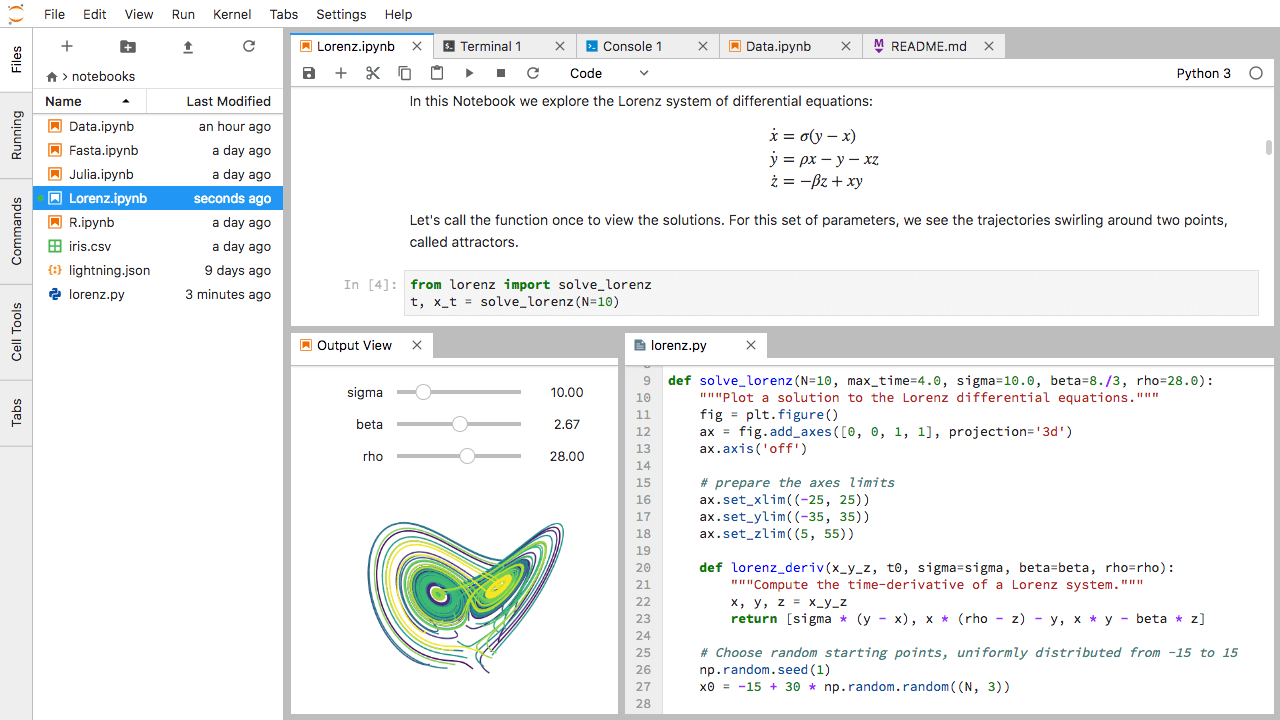
\includegraphics[width=\textwidth]{Images/jupyterlab.png}
	\caption{Interfaz gr\'afica de ejemplo desarrollada con Jupyter. Fuente: https://jupyterlab.readthedocs.io/en/latest/}
	\label{jupyter}
\end{figure}

\noindent
\justify

``Jupyter es una aplicaci\'on web de c\'odigo abierto que permite la creaci\'on y compartibilidad de diferentes documentos, encontr\'andose en ellos: c\'odigo \textit{en vivo}, ecuaciones y visualizaci\'on de texto explicativo. Entre sus usos se encuentran: limpieza y transformaci\'on de datos, simulaciones num\'ericas, modelado estad\'istico y aprendizaje autom\'atico, entre muchos otros." Descripci\'on oficial del proyecto Jupyter.

\noindent
\justify

Parte del Frontend desarrollado para brindar interactividad de usuario se puede apreciar en la Figura \ref{interfaz}.

\begin{figure}[h!]
	\centering
	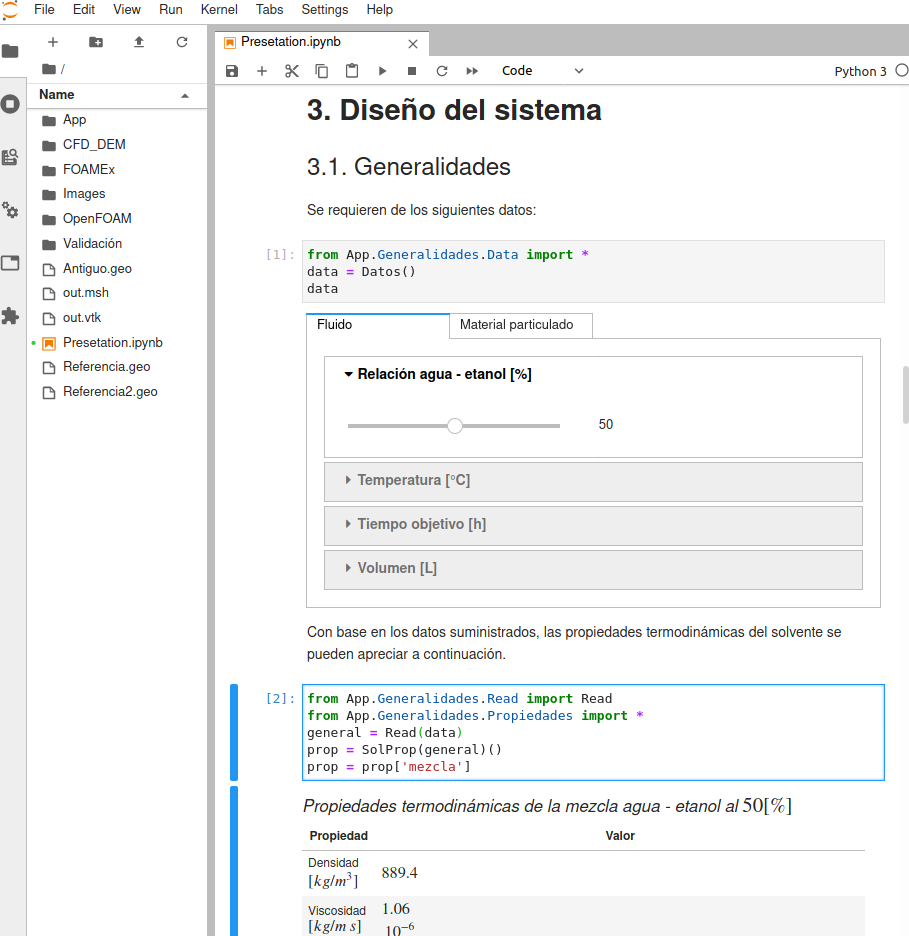
\includegraphics[width=\textwidth]{Images/interfaz.png}
	\caption{Parte de la interfaz gr\'afica desarrollada para la automatizaci\'on del modelo CFD-DEM.}
	\label{interfaz}
\end{figure}

\noindent
\justify


Jupyter permite la interactividad a trav\'es de diferentes lenguajes de Frontend; entre ellos: HTML, CSS y JavaScript. Para la escritura de textos, adopta lenguajes como Markdown y \LaTeX. Adem\'as, cuenta con diferentes librer\'ias internas para el desarrollo de contenidos interactivos, de las que se destacan: \texttt{ipywidgets}, \texttt{IPython.display} y \texttt{Plotly}. 

\begin{figure}[h!]
	\centering
	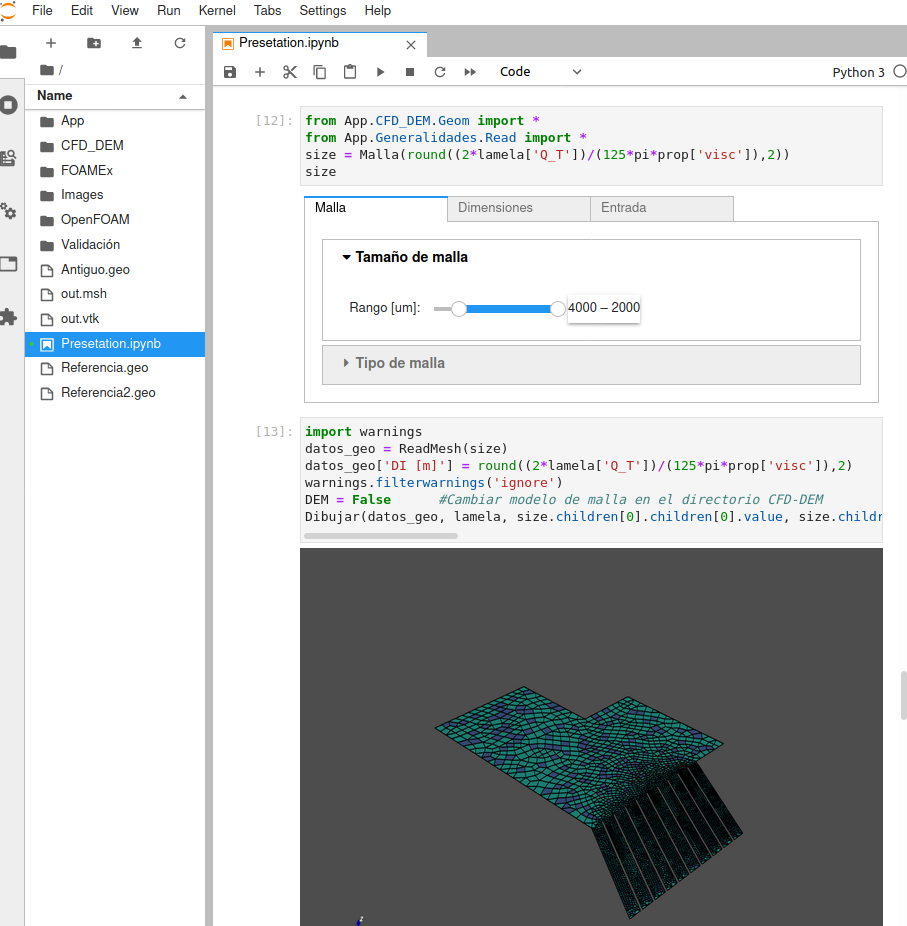
\includegraphics[width=\textwidth]{Images/interfaz2.png}
	\caption{Secci\'on de mallado autom\'atico del software desarrollado mediante \texttt{gmsh}.}
	\label{mallado:gmsh}
\end{figure}

\noindent
\justify

En la Figura \ref{mallado:gmsh} se puede apreciar la interfaz gr\'afica referente al mallado autom\'atico de la geometr\'ia, desarrollado en el lenguaje \texttt{gmsh}; en d\'onde el usuario puede definir el rango de tama\~no de malla, tipo de los elementos (rectangular o triangular) y las dimensiones de la geometr\'ia.

\newpage

\subsubsection{Backend}

\noindent
\justify

Detr\'as de la funcionalidad del software se encuentra el \'arbol de directorios mostrado en la Figura \ref{particion}.

\begin{figure}[h!]
\centering
\begin{forest}
  pic dir tree,
  where level=0{}{% folder icons by default; override using file for file icons
    directory,
  },
  [CFD-DEM Software
    [App
      [{CFD\_DEM}
        [CF.py, file
        ]
        [CFD.py, file
        ]
        [CFDEM.py, file
        ]
        [Geom.py, file
        ]        
        [Malla.py, file
        ]
      ]
      [Generalidades
        [Lamelas.py, file
        ]
        [Propiedades.py, file
        ]
        [Read.py, file
        ]
      ]
      [Sedimentaci\'on
        [Inicial.py, file
        ]      
        [ParOper.py, file
        ]
        [Resultados.py, file
        ]
      ]
    ]
    [{CFD\_DEM}
    ]
    [OpenFOAM
    ]
    [Validaci\'on
    ]
    [Presentation.ipynb, file
    ]
  ]
\end{forest}
\caption{\'Arbol de directorios.}
\label{particion}
\end{figure}

\newpage

\noindent
\justify

El software resuelve, b\'asicamente, tres problemas:

\begin{itemize}
	\item Dise\~no funcional del panel de lamelas desde un enfoque te\'orico.
	\item An\'alisis del comportamiento, a trav\'es de OpenFOAM, de la din\'amica de fluidos del panel de lamelas.
	\item Simulaci\'on CFD-DEM que permite predecir la interacci\'on fluido - part\'icula a distintas condiciones de flujo.
\end{itemize}

\paragraph{Dise\~no funcional te\'orico}

\noindent
\justify

El dise\~no funcional busca defnir una geometr\'ia inicial del panel de lamelas, para el an\'alisis consecuente mediante los m\'etodos num\'ericos de \textit{vol\'umenes finitos} y \textit{elementos discretos}, a trav\'es de metodolog\'ias te\'oricas y experimentales (cap\'itulo \ref{teorico:sed}).

\noindent
\justify

La l\'ogica desarrollada comprende los siguientes pasos:

\begin{enumerate}
	\item Definici\'on, por parte del usuario, de las propiedades del solvente (entre ellas: proporci\'on de la mezcla hidroetan\'olica) y del material particulado.
	\item C\'alculo de las propiedades termodin\'amicas del fluido.
	\item Definici\'on de la geometr\'ia del panel de lamelas.
	\item C\'alculo de las diferentes propiedades del solvente: caudal, velocidad del fluido y de la sedimentaci\'on y el n\'umero de Reynolds, por mencionar algunos.
\end{enumerate}

\noindent
\justify

Los algoritmos que emplean esta l\'ogica se encuentran ubicados en las direcciones \texttt{App/Sedimentaci\'on} y \texttt{App/Generalidades}, como se aprecia en la Figura \ref{particion}.

\paragraph{Simulaciones num\'ericas} \label{imp:CFD}

\noindent
\justify

El modelo CFD permite conocer el comportamiento del solvente dentro del volumen de control para contrastarlo con el modelo CFD-DEM. Comprende los siguientes pasos:

\begin{enumerate}
	\item Definici\'on de la geometr\'ia.
	\item Mallado de la geometr\'ia.
	\item Definici\'on de las condiciones de frontera.
	\item Desarrollo de la simulaci\'on.
	\item Postprocesamiento y presentaci\'on de resultados.
\end{enumerate}

\noindent
\justify

Los algoritmos desarrollados para el desarrollo de este modelo se encuentran ubicados en la direcci\'on \texttt{App/{CFD\_DEM}}:

\begin{itemize}
	\item \texttt{Geom.py} permite establecer la geometr\'ia del problema de acuerdo a los par\'ametros definidos por el usuario.
	\item \texttt{Malla.py} define el mallado de la geometr\'ia, ejecutando el lenguaje \textit{gmsh}.
	\item \texttt{CF.py} define las condiciones de frontera.
	\item \texttt{CFD.py} se encarga de ejecutar la simulaci\'on num\'erica a trav\'es de OpenFOAM.
\end{itemize}

\noindent
\justify

El modelo CFD-DEM predice las interacciones fluido-part\'icula del sistema de sedimentaci\'on. Emplea la misma l\'ogica descrita en la secci\'on \ref{imp:CFD}. La \'unica diferencia radica en la ejecuci\'on del algoritmo descrito en \texttt{CFD.py}; en su lugar, ejecuta el de \texttt{CFDEM.py} que contiene la metodolog\'ia de desarrollo de la simulaci\'on CFD-DEM basada en el m\'etodo Euler - Lagrange.


\begin{center}
	\section{Resultados} \label{teorico:sed}
\end{center}


\subsection{Propiedades del fluido}

\noindent
\justify

Las Ecuaciones \ref{rhoH2O} y \ref{viscH2O} describen las propiedades termodin\'amicas del agua; y las Ecuaciones \ref{rhoEt} y \ref{viscEt} las del etanol a presi\'on atmosf\'erica en funci\'on de la temperatura del fluido $\left(\forall T \, \varepsilon [5 \degree C, 60 \degree C] \right)$. La Ecuaci\'on \ref{mezcla} permite predecir las propiedades de la mezcla agua - etanol a cualquier grado de concentraci\'on. Las propiedades de una mezcla agua - etanol al $50 \%$, $28 [\degree C]$, se pueden apreciar en el Cuadro \ref{temoM}.

\begin{table}[h!]
	\centering
	\begin{tabular}{|c|c|}
	\hline
	\textbf{Propiedad} & \textbf{Valor} \\ \hline
	$\rho _f \left[ kg / m^3 \right]$ & $889.4$ \\ \hline
	$\mu _f \left[ m^2 / s \right] $ & $1.06 * \, 10^{-6}$ \\ \hline
	\end{tabular}
	\caption{Propiedades de la mezcla agua - etanol al $50 \%$.}
	\label{temoM}
\end{table}

\subsection{Velocidad m\'axima de sedimentaci\'on}

\noindent
\justify

La velocidad m\'axima de sedimentaci\'on se calcula a trav\'es del procedimiento iterativo mostrado en la Figura \ref{UmaxS}. Los resultados de este procedimiento se pueden apreciar en la Figura \ref{iteraciones}.

\begin{table}[h!]
	\centering
	\begin{tabular}{|c|c|c|c|c|c|}
	\hline
	Iteraci\'on & $U_s [m/s]$ & $Re_s$ & $C$ & $U_c [m/s]$ & $Err_c [\%]$ \\ \hline
	1 & $1$ & $236.247$ & $0.637$ & $0.068$ & $93.159$ \\ \hline
	2 & $0.068$ & $16.162$ & $2.571$ & $0.034$ & $50.235$ \\ \hline
	3 & $0.034$ & $8.043$ & $4.382$ & $0.026$ & $23.397$ \\ \hline
	\multicolumn{6}{|c|}{$\cdots$} \\ \hline
	13 & $0.022$ & $5.115$ & $6.359$ & $0.022$ & $0.04 \, *10^{-1}$ \\ \hline	
	\end{tabular}
	\caption{Proceso de c\'alculo iterativo de la velocidad de sedimentaci\'on m\'axima.}
	\label{iteraciones}
\end{table}

\noindent
\justify

Se concluye que, con una estimaci\'on de error inferior al $0.01 \%$, la velocidad m\'axima de sedimentaci\'on es de $0.022 [m/s]$ con un n\'umero de Reynolds en la part\'icula de $5.115$.

\subsection{Geometr\'ia inicial}

\noindent
\justify

Con base en lo descrito en las secciones \ref{geoLa}, \ref{anchoSed}, \ref{Rev0} y \ref{enTol} la geometr\'ia del sistema de sedimentaci\'on de placas inclinadas presenta las siguientes dimensiones:

\begin{table}[h!]
	\centering
	\begin{tabular}{|c|c|}
		\hline
		\textbf{Par\'ametro} & \textbf{Valor} \\ \hline
			Ancho lamela $[cm]$ & $5$ \\ \hline
			Longitud lamela $[cm]$ & $40$ \\ \hline
			Separaci\'on entre lamelas $[cm]$ & $2.5$ \\ \hline
			Inclinaci\'on $[\degree]$ & $60$ \\ \hline
			N\'umero lamelas & $5$ \\ \hline
			Ancho panel $[cm]$ & $2.2$ \\ \hline
			Di\'ametro de entrada $[cm]$ & $27$ \\ \hline
			Altura total $[cm]$ & $105$ \\ \hline
	\end{tabular}
	\caption{Geometr\'ia de estudio}
	\label{GeoInicial}
\end{table}

\noindent
\justify

Es posible apreciar la geometr\'ia de an\'alisis en la Figura \ref{geometry}; destacando: una zona de \textit{entrada} de la mezcla s\'olido - l\'iquido; una de \textit{salida} (al final de la superficie inclinada), en donde se espera obtener la \textit{fase l\'iquida} de la mezcla y un \'area de dep\'osito de lodos, localizada en la parte inferior de la geometr\'ia. El \textbf{\'area sombreada} corresponde a la regi\'on de inter\'es en donde se desarrollan las simulaciones num\'ericas.

%Datos geométricos
\def\D{2.7}    	%Diámetro de ingreso
\def\H{3}		%Altura de la zona de lodos
\def\A{2.5}		%Ancho del panel de lamelas
\def\HL{3}		%Altura del panel de lamelas
\def\nL{5}		%Número de lamelas
\def\ang{60}	%Ángulo de inclinación del panel

\def\xlam{\x+\A+0.5*\D}

\def\fin{\nL-1}

%Inclinación
%\def\xL{{\HL*cos(\ang)}}

%Referencia
\def\x{-\A/2-0.5/2*\D-\HL/2}
\def\y{0}

\begin{figure}[h!]
	\centering
	\begin{adjustbox}{max width = \textwidth}
	\begin{tikzpicture}
		%Geometría general
		\draw (\x,\y) -- (\x,-\D) -- (\x+0.5*\D,-\D) --
			(\x+0.5*\D, -2*\D) -- ({\x+0.5*\D + \A/3}, -2.5*\D) -- ({\x+0.5*\D + 2*\A/3}, -2.5*\D) -- (\x+\A+0.5*\D, -2*\D) -- 
			(\x+\A+0.5*\D, \y) -- ({\xlam + \HL*cos(\ang)},{\y + \HL*sin(\ang)}) -- ({\xlam + \HL*cos(\ang) - \A}, {\y + \HL*sin(\ang)}) -- (\xlam - \A, \y) -- cycle;
						
		%Lamelas
		\foreach \xL in {1, ..., \nL}
			\draw (\xlam - \xL*\A/\nL,\y) -- ({\xlam + \HL*cos(\ang) - \xL*\A/\nL}, {\y + \HL*sin(\ang)});
		\foreach \xL in {1, ..., \nL}	
			\draw[dashed, step=0.5cm, blue!60!green, pattern=north west lines, pattern color=blue!60!green] ({\xlam - (\xL-1)*\A/\nL},\y) -- (\xlam - \xL*\A/\nL,\y) -- ({\xlam + \HL*cos(\ang) - \xL*\A/\nL}, {\y + \HL*sin(\ang)}) -- ({\xlam + \HL*cos(\ang) - (\xL-1)*\A/\nL}, {\y + \HL*sin(\ang)})  -- cycle;
			
		%Dimensiones
		\draw (\x+0.5*\D + 0.1, -2*\D) -- (\x, -2*\D);
		\draw[arrows={-Triangle[angle=90:3pt,red!10!black,fill=red!10!black]}] (\x+0.25*\D, -2*\D) -- (\x+0.25*\D, -\D);
		\draw[arrows={-Triangle[angle=90:3pt,red!10!black,fill=red!10!black]}] (\x+0.25*\D, -\D)  -- (\x+0.25*\D, -2*\D);
		\node[align=left] at (\x-0.1, -3/2*\D) {$29.4 [cm]$};
		
		\draw (\x+0.5*\D + 0.1 + \A, -2*\D) -- (\x+\D + 0.1 + \A, -2*\D);
		\draw (\x+0.5*\D + 0.1 + \A, \y) -- (\x+1.5*\D + 0.1 + \A, \y);
		
		\draw[arrows={-Triangle[angle=90:3pt,red!10!black,fill=red!10!black]}] (\x+0.75*\D + \A, -2*\D) -- (\x+0.75*\D+ \A, \y);
		\draw[arrows={-Triangle[angle=90:3pt,red!10!black,fill=red!10!black]}] (\x+0.75*\D+ \A, \y) --  (\x+0.75*\D+ \A, -2*\D);
		
		\node[align=right] at (\x+1.05*\D+ \A, -\D) {$56.4 [cm]$};
		
		\draw ({\xlam + \HL*cos(\ang)},{\y + \HL*sin(\ang)}) -- ({\xlam + \HL*cos(\ang) + \D},{\y + \HL*sin(\ang)});

		\draw (\x+0.5*\D, -2*\D - 0.1) -- (\x+0.5*\D, -2.8*\D - 0.1);
		\draw (\x+0.5*\D + \A, -2*\D - 0.1) -- (\x+0.5*\D + \A, -2.8*\D - 0.1);	
		\draw[arrows={-Triangle[angle=90:3pt,red!10!black,fill=red!10!black]}] (\x+0.5*\D + \A, -2.6*\D-0.1) -- (\x+0.5*\D, -2.6*\D - 0.1);
		\draw[arrows={-Triangle[angle=90:3pt,red!10!black,fill=red!10!black]}] (\x+0.5*\D, -2.6*\D - 0.1) -- (\x+0.5*\D + \A, -2.6*\D-0.1);
		
		\node at (\x+0.5*\D + \A/2, -2.7*\D - 0.1) {$35 [cm]$};	
		
		\draw[arrows={-Triangle[angle=90:3pt,red!10!black,fill=red!10!black]}] ({\xlam + \HL*cos(\ang) + \D/4}, {\y + \HL*sin(\ang)}) -- ({\xlam + \HL*cos(\ang) + \D/4}, \y);
		
		\draw[arrows={-Triangle[angle=90:3pt,red!10!black,fill=red!10!black]}] ({\xlam + \HL*cos(\ang) + \D/4}, \y) --  ({\xlam + \HL*cos(\ang) + \D/4}, {\y + \HL*sin(\ang)});
		
		\node at ({\xlam + \HL*cos(\ang) + \D/4 + 0.75}, {\y + \HL*sin(\ang)/2}) {$34.6 [cm]$};
		
		%Área de interés
		\draw[dashed, step=0.5cm, blue!60!green, pattern=north west lines, pattern color=blue!60!green] (\x,\y) -- (\x,-\D) -- (\x+0.5*\D,-\D) -- (\x+0.5*\D, -2*\D) -- (\x+\A+0.5*\D, -2*\D) -- (\x+\A+0.5*\D, \y) -- cycle;
		
		%Señalización
		\draw[red!10!black, arrows={-Triangle[angle=90:3pt,red!10!black,fill=red!10!black]}] (\x-2,-\D/2) node[above] {Entrada \textit{mezcla}} -- (\x-0.5,-\D/2);
		
		\draw[red!10!black, arrows={-Triangle[angle=90:3pt,red!10!black,fill=red!10!black]}] ({\xlam + \HL*cos(\ang) - \A/\nL/2},{\y + \HL*sin(\ang)}) node[above] {Salida \textit{fase l\'iquida}} -- ({\xlam + (\HL+1)*cos(\ang) - \A/\nL/2},{\y + (\HL+1)*sin(\ang)});
		
		
	\end{tikzpicture}
	\end{adjustbox}
	\caption{Vista en corte de la geometr\'ia del sistema de sedimentaci\'on.}
	\label{geometry}
\end{figure}

\noindent
\justify

Con base en la geometr\'ia descrita en el Cuadro \ref{GeoInicial}, se obtuvieron los siguientes par\'ametros operacionales:

\begin{itemize}
	\item $v_0 = 1.014 [cm/s]$
	\item $Re = 478.993$
	\item $U_c = 0.208 [cm/s]$
\end{itemize}

\subsection{Mallado}

\noindent
\justify

Gran parte del \'exito de las simulaciones num\'ericas recaen en la discretizaci\'on del dominio y en la calidad de los elementos que la componen$^{\cite{Roda-Casanova2021}}$. Se desarroll\'o una metodolog\'ia de mallado autom\'atico con base en el lenguaje \textit{gmsh} tomando como variables de entrada las dimensiones de la geometr\'ia definida en la secci\'on \ref{geo}. Esta metodolog\'ia emplea elementos de diferentes tama\~nos y permite tambi\'en definir su naturaleza (rectangulares o triangulares).

\noindent
\justify

El algoritmo ejecuta, adem\'as, un refinamiento autom\'atico en la zona en donde ocurre el mayor grado de sedimentaci\'on: en la superficie inclinada, como se aprecia en la Figura \ref{malla:geo}.

\begin{figure}[h!]
	\centering
	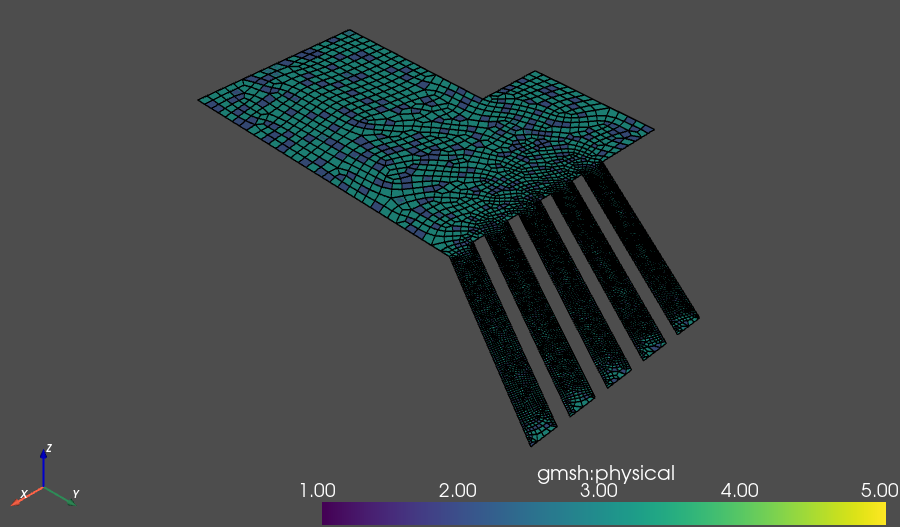
\includegraphics[width=\textwidth]{Images/CFDEM/malla2.png}
	\caption{Mallado de la geometr\'ia.}
	\label{malla:geo}
\end{figure}

\newpage

\noindent
\justify

La malla mostrada en la Figura \ref{malla:geo} presenta las siguientes caracter\'isticas:

\begin{table}[h!]
	\centering
	\begin{tabular}{|c|c|}
		\hline
		\textbf{Par\'ametro} & \textbf{Valor} \\ \hline
		Tipo de elementos & Rectangulares \\ \hline
		N\'umero de elementos & 20415 \\ \hline
		N\'umero de nodos & 13692 \\ \hline	
	\end{tabular}
	\caption{Datos de la malla generada.}
	\label{malla}
\end{table}

\noindent
\justify

Al emplear el m\'etodo \texttt{checkMesh} de OpenFOAM para el an\'alisis preliminar de malla, se obtuvieron los siguientes resultados:

\begin{table}[h!]
	\centering
	\begin{tabular}{|c|c|}
		\hline
		\textbf{Par\'ametro} & \textbf{Valor} \\ \hline
		Apertura \textit{m\'axima} entre elementos & 11.45 \\ \hline
		Checkeo de \textit{no} ortogonalidad & OK \\ \hline
		Oblicuidad m\'axima & 0.66 OK \\ \hline
		Conclusi\'on de malla & OK \\ \hline
	\end{tabular}
	\caption{Resumen de resultados sobre el checkeo de malla.}
	\label{check}
\end{table}

\noindent
\justify

A partir de los resultados mostrados en el Cuadro \ref{check}, se concluye que la malla es \'optima para el desarrollo de las simulaciones num\'ericas consecutivas.

\subsection{Condiciones de frontera}

\noindent
\justify

Complementando la informaci\'on descrita en la secci\'on \ref{CondF}, las condiciones de frontera del problema se resumen en el Cuadro \ref{condFr}.

\begin{table}[h!]
	\centering
	\begin{tabular}{|c|c|c|c|}
		\hline
		\textbf{Zona} & \textbf{Propiedad} & \textbf{Valor}  & \textbf{Tipo} \\ \hline
		\textit{Entrada} & Velocidad $[m/h]$ & $3.493$ & Neumann \\ \hline
		\textit{Salida} & Presi\'on $[KPa]$ & $101.325$ & Dirichlet \\ \hline
	\end{tabular}
	\caption{Clasificaci\'on de las condiciones de frontera.}
	\label{condFr}
\end{table}

\newpage

\subsection{Simulaci\'on CFD}

\noindent
\justify

Con base en la metodolog\'ia descrita en la secci\'on \ref{MetCFD}, se emple\'o el solucionador \texttt{pimpleFOAM} de OpenFOAM; obteniendo los siguientes resultados:

\begin{figure}[h!]
	\centering
	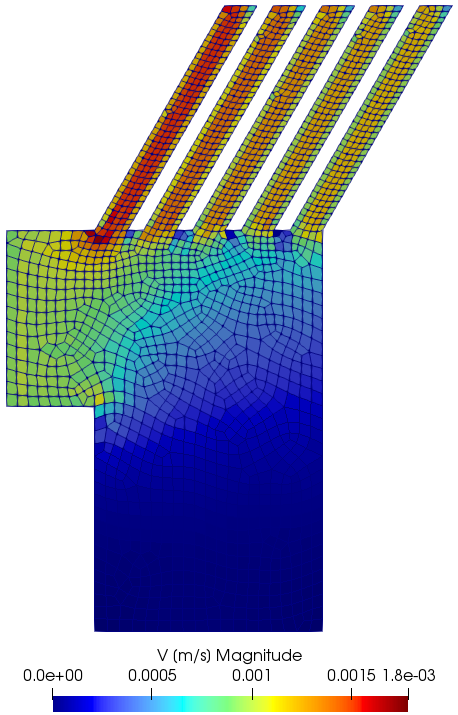
\includegraphics[width=0.33\textwidth]{Images/CFD/vel1.png}
	\caption{Diagrama de contorno de la distribuci\'on de velocidades del sistema de sedimentaci\'on.}
	\label{CFD:vel}
\end{figure}

\begin{figure}[h!]
	\centering
	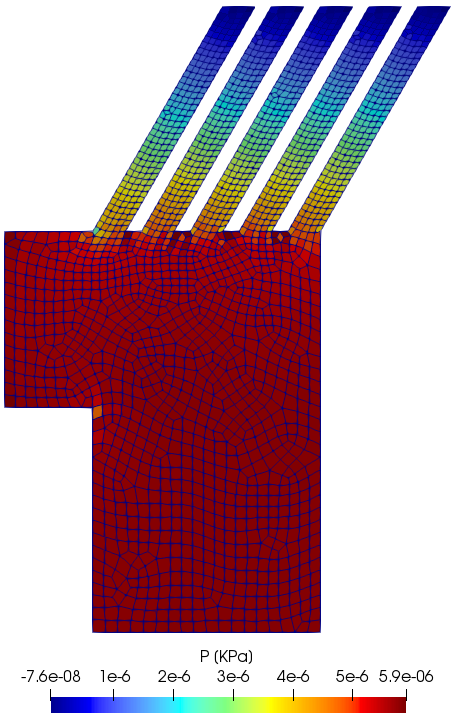
\includegraphics[width=0.33\textwidth]{Images/CFD/p1.png}
	\caption{Diagrama de contorno de la distribuci\'on de presiones del sistema de sedimentaci\'on.}
	\label{CFD:p}
\end{figure}

\subsection{Error computacional}

\noindent
\justify

De acuerdo a lo estipulado en la secci\'on \ref{errorSimu}, se desarroll\'o un refinamiento de malla para calcular el error de la simulaci\'on num\'erica debido a la calidad de malla. El resumen de resultados se puede apreciar en el Cuadro \ref{resumErr}.

\begin{table}[h!]
	\centering
	\begin{tabular}{|c|c|c|c|}
		\hline
		\textbf{Iteraci\'on} & \textbf{N\'um. nodos} & \textbf{Vel. m\'ax.$[m/s]$} & \textbf{P. m\'ax. $[KPa]$} \\ \hline
		1 & $4560$ & $0.0017$ & $6.5 \, \cdot 10 ^{-6}$ \\ \hline
	\end{tabular}
	\caption{Resultados del proceso iterativo.}
	\label{resumErr}
\end{table}

\noindent
\justify

En la Figura \ref{resumErrG}, se puede apreciar la tendencia 
\begin{center}
	\section{An\'alisis de resultados}
\end{center}

\noindent
\justify

La simulaci\'on num\'erica CFD, desarrollada con el solucionador \texttt{pimpleFoam}, de OpenFOAM, encontr\'o su punto de equilibrio (punto \textit{estacionario}) al cabo de ocho segundos de simulaci\'on. En la Figura \ref{CFD:vel} se observa un valor de velocidad m\'axima de $0.0018 [m/s]$ que es alcanzado en la primera lamela y decrece en las lamelas consecuentes hasta un valor cercano de $0.0012 [m/s]$; fen\'omeno f\'isico que va acorde a la realidad por tratarse de flujos en serie.

\noindent
\justify

En la Figura \ref{CFD:p} se puede apreciar el perfil de presiones sobre el sistema; en donde se presenta un comportamiento uniforme y sim\'etrico alcanzando un valor de presi\'on m\'axima de hasta $5.90 \cdot 10^{-6} [kPa]$. Como era de esperarse, las condiciones de frontera establecidas en la secci\'on \ref{CondF} fueron respetadas: en la salida del flujo se aprecia una presi\'on manom\'etrica de $0 [KPa]$ (atmosf\'erica) y la velocidad de flujo en la entrada es de $0.00097 [m/s] \approx 3.493 [m/h]$.

\noindent
\justify

Comparando las Figuras \ref{CFD:vel} y \ref{CFDEM:vel}, se puede apreciar c\'omo el solvente cambia la distribuci\'on de velocidades por la sedimentaci\'on sufrida por las part\'iculas de arena, cuya densidad es mayor que la del fluido circundante; raz\'on por la que el solvente tiende a moverse con mayor velocidad en las \'ultimas lamelas en lugar de las primeras, a diferencia de lo observado en la secci\'on \ref{CFD:resultados}. Debido a ello, es posible clasificar a las lamelas por zonas de \textit{``pureza"} durante el proceso de separaci\'on: en donde las primeras cuatro presentan menor concentrac\'on particular que las \'ultimas cuatro.

\noindent
\justify

La presencia de v\'ortices y remolinos en la simulaci\'on CFD-DEM rectifica la decisi\'on de haber empleado un solucionador basado en \texttt{pimpleFoam}, el cual fue adaptado para resolver el problema \textit{Euler - Lagrange} (E - L).

\noindent
\justify

Diferente al fen\'omeno apreciado en la Figura \ref{CFD:p}, la distribuci\'on de presiones en la Figura \ref{CFDEM:p} no es sim\'etrica y tiende a presentar sus m\'aximos valores en la zona de congregaci\'on de los sedimentos.

\begin{figure}[h!]
	\centering
	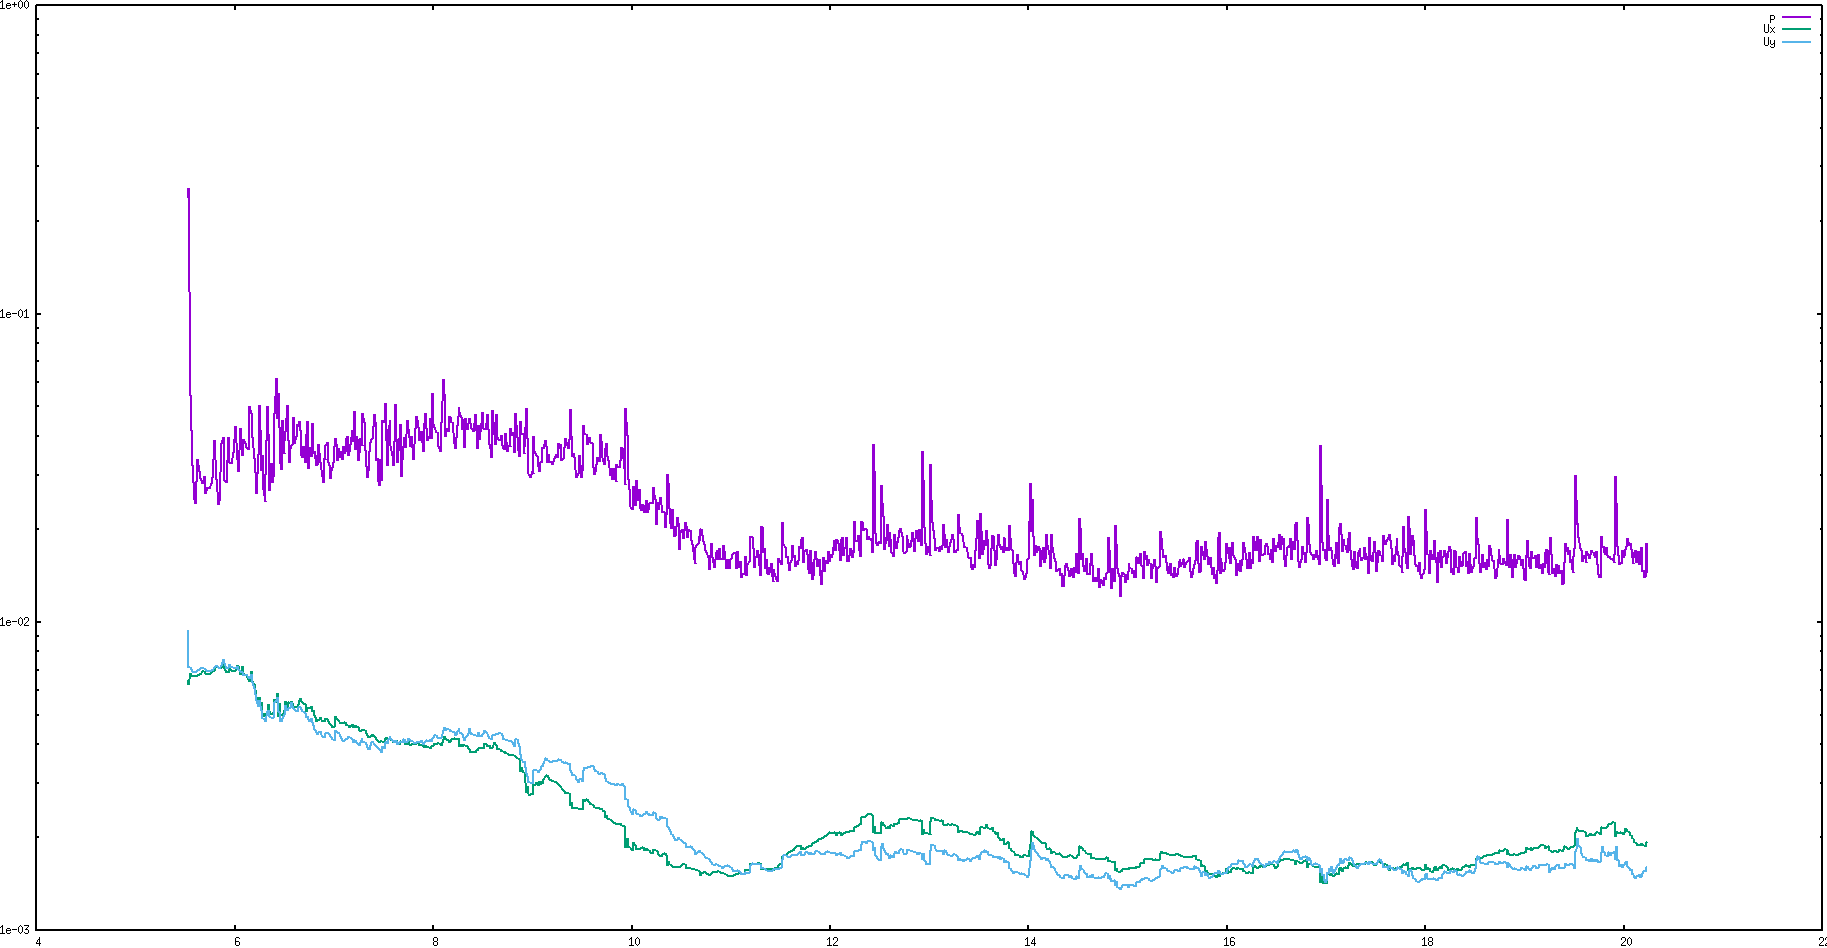
\includegraphics[width=\textwidth]{Images/CFDEM/residuals.png}
	\caption{Monitoreo de residuales en la simulaci\'on CFD-DEM.}
	\label{CFDEM:residuals}
\end{figure}

\noindent
\justify

De la Figura \ref{CFDEM:residuals}, la l\'inea morada corresponde al residual de la presi\'on, la de color cian al residual de la velocidad en $y$ y la de color verde al residual de la velocidad en $x$. El comportamiento de los residuales est\'a directamente relacionado con la magnitud de los errores en la soluci\'on de las ecuaciones gobernantes$^{\cite{Liang2018}}$. 

\newpage

\noindent
\justify

Debido al hecho de que los residuales tienden a aglomerarse en valores cercanos a cero, son un indicativo de alta precisi\'on del modelo num\'erico implementado. Las variaciones vistas en los residuales de presi\'on se deben a la vorticidad originada por los reflujos consecuentes a la interacci\'on fluido - part\'icula. Durante la simulaci\'on, se observ\'o una estabilizaci\'on en los perfiles de velocidad; raz\'on por la que los residuales $U_x$ y $U_y$ presentan un comportamiento sin fluctuaciones y con peque\~nas variaciones durante el desarrollo del flujo dentro del volumen de control.
\begin{center}
    \section{Validaci\'on del modelo}
\end{center}

\noindent
\justify

Para la validaci\'on del modelo CFD-DEM desarrollado, se aplic\'o el modelo para resolver el problema de Fessler \& Eaton$^{\cite{Fessler1999}}$, en donde se investig\'o el efecto de la turbulencia generada por part\'iculas de cobre de $70 [\mu m]$ de di\'ametro sobre un flujo \textit{orientado hacia atr\'as}, como se muestra en la Figura \ref{problemaVal}.

\begin{figure}[h!]
    \centering
    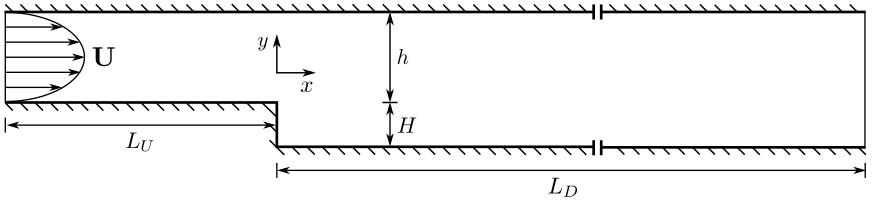
\includegraphics[width=0.75\textwidth]{Images/Fessler.PNG}
    \caption{Geometr\'ia de estudio.}
    \label{problemaVal}
\end{figure}

\subsection{Descripci\'on del problema}

\noindent
\justify

En 1999, Fessler \& Eaton estudiaron el efecto de part\'iculas de vidrio y cobre de distintos tama\~nos ($70$, $90$ y $150 [\mu m]$ de di\'ametro), a diferentes cargas m\'asicas (entre el 3 y el 40 \% del flujo m\'asico) y a las mismas condiciones experimentales de velocidad y presi\'on en donde se apreci\'o una atenuaci\'on del flujo relacionada con un decaimiento en el n\'umero de Stokes de las part\'iculas.

\noindent
\justify

La motivaci\'on detr\'as de esta investigaci\'on recae en la complejidad de las interacciones entre part\'iculas peque\~nas y densas con la fase turbulenta de una sustancia gaseosa; adem\'as de la importancia en diferentes casos, de car\'acter industrial y natural, en donde se producen flujos particulados que son, muchas veces, inentendidos. En pocos aspectos, tales como la dispersi\'on de part\'iculas en flujos homog\'eneos, se pueden llevar a cabo estudios anal\'iticos con altos niveles de precisi\'on. Sin embargo, la mayor\'ia de los casos en la realidad comprenden flujos heterog\'eneos y anisotr\'opicos sujetos a inestabilidades, con marcadas variaciones entre flujo y flujo, que imposibilitan el desarrollo de un modelo matem\'atico anal\'itico que defina a cabalidad la naturaleza de los flujos y que sea, a su vez, lo suficientemente preciso. 

\noindent
\justify

Se ha reportado en la literatura que los niveles de turbulencia pueden ser moderados con la ayuda de la carga de diferentes masas. Investigaciones como la de Hetsroni$^{\cite{Hetsroni1989}}$ y Gore \& Crowe$^{\cite{Gore1991}}$ establecieron los cimientos del comportamiento turbulento en la interacci\'on fluido - part\'icula; mientras que en investigaciones desarrolladas por Kulick, Fessler \& Eaton$^{\cite{Kulick1994}}$ y Tsuji, Morikawa \& Shiomi$^{\cite{Tsuji1984}}$ se demostr\'o que la atenuaci\'on de la turbulencia incrementa tanto con la carga m\'asica como con el n\'umero de Stokes de las part\'iculas.  

\noindent
\justify

En el presente estudio se investig\'o el comportamiento de las part\'iculas sobre un flujo \textit{orientado hacia atr\'as} (Figura \ref{problemaVal}). Este flujo es ideal para el estudio de la interacci\'on part\'icula-turbulencia debido a que las estad\'isticas del flujo medio son conocidas como \textit{invariables} debido a la presencia de part\'iculas s\'olidas$^{\cite{Kulick1994}}$; hecho esencial que garantiza que los cambios en la turbulencia se deben \'unicamente a la presencia de material particulado, dado que los flujos separados son sensibles al perfil de velocidad media. En este trabajo se emplearon part\'iculas de vidrio de $90$ y $150 [\mu m]$ de di\'ametro y part\'iculas de cobre de $70 [\mu m]$; que proveen dos diferentes part\'iculas con n\'umeros de Stokes distinto y tres diferentes valores de Reynolds. 

\begin{table}[h!]
	\centering
	\begin{tabular}{|c|c|}
		\hline
		\textbf{Par\'ametro} & \textbf{Valor} \\ \hline
		Altura $H$ & $26.7 [mm]$ \\ \hline
		Rango de expansi\'on & 5:3 \\ \hline
		Relaci\'on de aspecto & 17:1 \\ \hline
		Velocidad inicial $U_0$ & $9.39 [m/s]$ \\ \hline
		$Re_H = \frac{U_0 H}{\mu}$ & $18400$ \\ \hline
		$\tau _f$, gran escala de tiempos de remolino, $\frac{5H}{U_0}$ & $12.7 [ms]$ \\ \hline
	\end{tabular}
	\caption{Par\'ametros del flujo.}
	\label{dataFlow}
\end{table}

\noindent
\justify

\subsection{Desarrollo experimental}

\noindent
\justify

El flujo sufre una expansi\'on unidireccional en donde se evita la sedimentaci\'on de part\'iculas. El n\'umero de Reynolds de la entrada fue de $13800$ con una velocidad en la l\'inea central de $10.5 [m/s]$. El rango de expansi\'on fue de $\frac{5}{3}$; mientras que la relaci\'on de aspecto es de 17:1. Hecho que garantiza un flujo bidimensional a trav\'es de una porci\'on importante del experimento.

\noindent
\justify

El condicionamiento del flujo de entrada, el flujo de salida y el sistema de alimentaci\'on de part\'iculas se ilustra en la Figura \ref{experimento}. El sistema provee velocidad de flujo uniforme con carga de part\'iculas en la entrada. Un canal de $5.2 [m]$ asegura el completo desarrollo del flujo y contempla el tiempo suficiente para que las part\'iculas lleguen al equilibrio con el medio circundante. Se emple\'o un ventilador, con frecuencia variable, como sistema de control m\'asico.

\begin{figure}[h!]
	\centering
	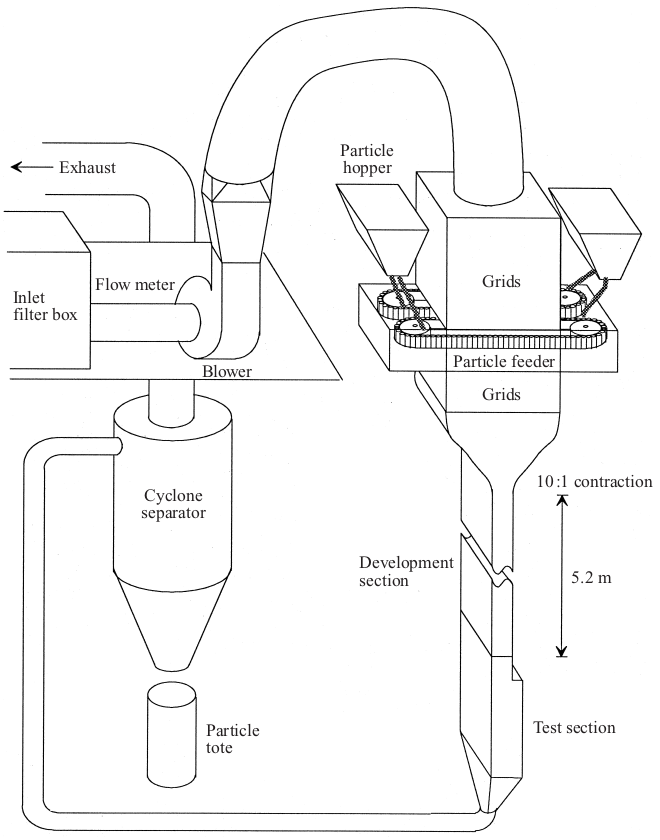
\includegraphics[width=0.7\textwidth]{Images/experimento.png}
	\caption{Esquema del montaje experimental$^{\cite{Fessler1999}}$.}
	\label{experimento}
\end{figure}

\subsubsection{Descripci\'on particular}

\noindent
\justify

El n\'umero de Reynolds que define el movimiento particular est\'a definido por la Ecuaci\'on \ref{Rep}.

\begin{equation}
	Re_p = \frac{d_p U_{rel}}{\mu}
	\label{Rep}
\end{equation}

\noindent
\justify

De la Ecuaci\'on \ref{Rep}: $d_p$ es el di\'ametro de la part\'icula, $\mu$ es la viscosidad cinem\'atica y $U_{rel}$ es la escala de velocidad que caracteriza la velocidad de deslizamiento medio de la part\'icula sobre el flujo.

\noindent
\justify

El n\'umero de Stokes es la relaci\'on entre el tiempo de respuesta de las part\'iculas con respecto a la escala de tiempo representativa en el flujo.

\begin{equation}
	St = \frac{\tau _p}{\tau _f}
	\label{Stp}
\end{equation}

\noindent
\justify

Para part\'iculas peque\~nas con n\'umeros de Reynolds despreciables, Stokes (1851) demostr\'o que la constante de tiempo particular se define con base en la Ecuaci\'on \ref{Stps}.

\begin{equation}
	\tau _{p, Stokes} = \frac{\left(2 \rho _p + \rho _f \right) d_p ^2}{36 \mu}
	\label{Stps}
\end{equation}

\noindent
\justify

El coeficiente de arrastre $C_D$, para n\'umeros de Reynolds superiores a $700$, puede calcularse con base en la Ecuaci\'on \ref{CD_700}.

\begin{equation}
	C_D = \frac{24}{Re_p} \left(1 + 0.15 Re_p ^{0.687} \right)
	\label{CD_700}
\end{equation}

\noindent
\justify

El incremento en el coeficiente de arrastre como el del n\'umero de Reynolds disminuir\'a la constante de tiempo particular; de modo que la constante de tiempo modificada empleada en este estudio se puede apreciar en la Ecuaci\'on \ref{taup}.

\begin{equation}
	\tau _p = \frac{\tau _{p, stokes}}{1 + 0.15 Re_p ^{0.687}}
	\label{taup}
\end{equation}

\noindent
\justify

La escala de tiempo representativa en el flujo se calcul\'o con base en la Ecuaci\'on \ref{tauf}.

\begin{equation}
	\tau _f = \frac{5H}{U_0}
	\label{tauf}
\end{equation}

\subsubsection{M\'etodos experimentales}

\noindent
\justify

Todas las velocidades de flujo fueron medidas a trav\'es de un anem\'ometro l\'aser Doppler (LDA, por sus siglas en ingl\'es). Cada punto de dato representa 2000 muestras individuales de velocidad que mantiene la incertidumbre estad\'istica desde $\pm 0.02 [m/s]$ hasta $\pm 0.08 [m/s]$. Para medir la velocidad de las part\'iculas, se emple\'o una t\'ecnica de discriminaci\'on por amplitud de pedestal, apreciable en la Figura \ref{medicion}. A partir de all\'i, se estim\'o un error experimental cercano al $5\%$. 

\begin{figure}[h!]
	\centering
	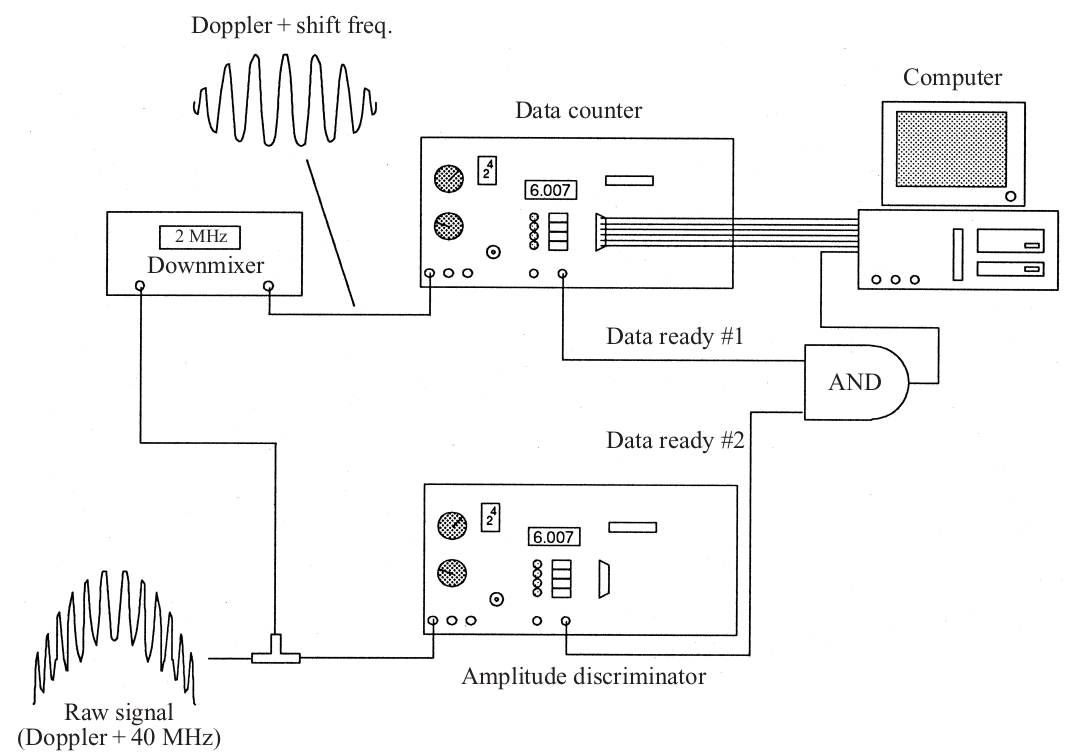
\includegraphics[width=0.68\textwidth]{Images/pedestal.png}
	\caption{Esquema del sistema de medici\'on de la interacci\'on part\'icula fluido$^{\cite{Fessler1999}}$.}
	\label{medicion}
\end{figure}

\noindent
\justify

El campo de densidad medio de part\'iculas se midi\'o al iluminar el material particulado a trav\'es de un pulso de frecuencia doble, $10 [mJ]$ por pulso de Neodimio, y al analizar diversas fotograf\'ias del experimento a trav\'es de un software de procesamiento de im\'agenes; permitiendo as\'i identificar cada part\'icula, su tama\~no y posici\'on en el lecho fluidizado.

\subsection{Resultados}

\noindent
\justify

Los perfiles de velocidad media se midieron, de manera experimental, a trav\'es de las condiciones especificadas en el Cuadro \ref{perfiles}. Pocas part\'iculas fueron identificadas en la zona de recirculaci\'on, por lo que no se reportaron datos en la zona $x/H = 2.5$ y $7$.

\begin{table}[h!]
	\centering
	\begin{adjustbox}{max width = \textwidth}
	\begin{tabular}{c c c c c}
		 & \multicolumn{2}{c}{\textbf{Direcci\'on de flujo}} & \multicolumn{2}{c}{\textbf{Direcci\'on normal al muro}} \\ \cmidrule{2-3}\cmidrule{4-5}
		 Clase de part\'icula & $x/H$ & Carga m\'asica & $x/H$ & Carga m\'asica \\ \hline
		 Vidrio de $90 [\mu m]$ & 2,5,7,9,14 & $20\%$ &  &  \\
		 Vidrio de $150 [\mu m]$ & 2,5,7,9,14 & $20\%, 40\%$ & 2,5,7,9,14 & $10\%$ \\
		 Cobre de $70 [\mu m]$ & -2, 0, 2, 5, 7, 9, 12 & $3\%, 10\%$ & 2,5,7,9,14 & $20\%$ \\
	\end{tabular}
	\end{adjustbox}
	\caption{Condiciones experimentales.}
	\label{perfiles}
\end{table}

\noindent
\justify

En la Figura \ref{resul1999} $a)$ se muestra el esquema de contorno de la densidad media de part\'iculas de cobre de $70 [\mu m]$. La velocidad m\'axima encontrada en este es, aproximadamente, de $0.2 U_0$. En la Figura \ref{resul1999} $b)$, se puede apreciar el esquema de contorno obtenido con base en el modelo CFD-DEM desarrollado.

\noindent
\justify

Cerca de la zona de salida del volumen de control, las velocidades de las part\'iculas exceden a las del gas debido a la desaceleraci\'on del fluido producida por la expansi\'on. La velocidad media de las part\'iculas en la direcci\'on del muro fue, generalmente, similar a las velocidades del fluido correspondiente.


\newpage

\begin{figure}[h!]
	\centering
	\begin{subfigure}[b]{\textwidth}
		\centering
		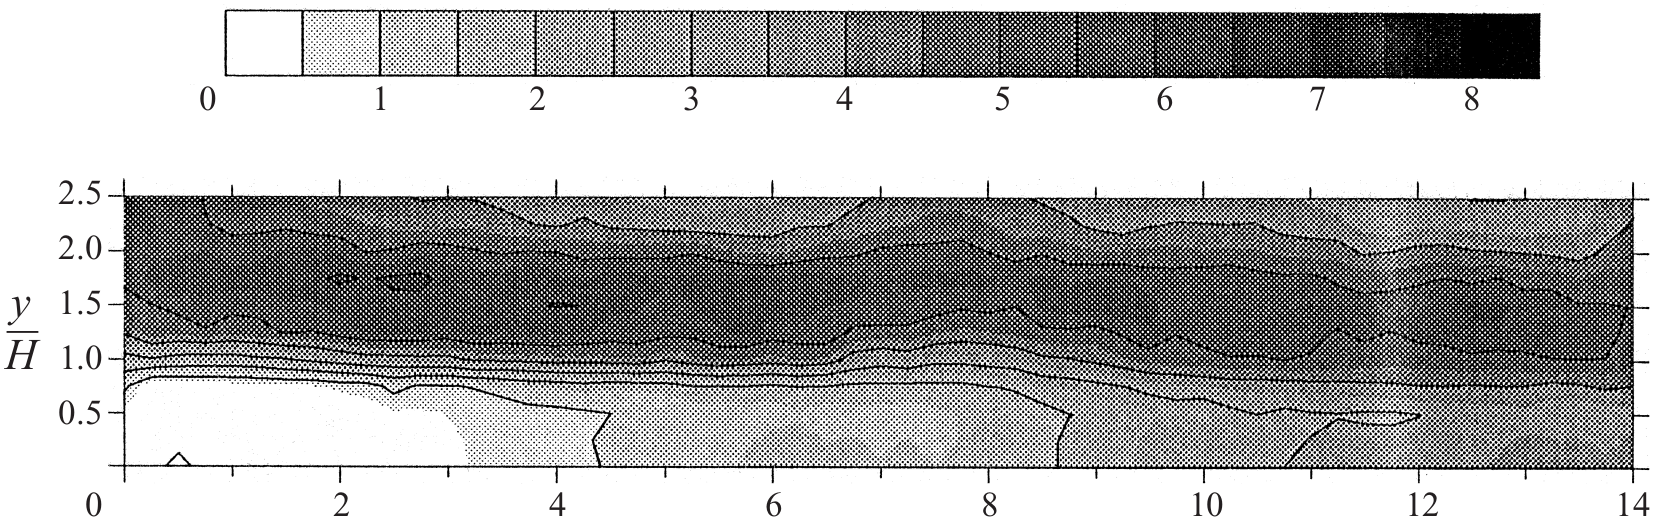
\includegraphics[width=\textwidth]{Images/contour1999.png}
		\caption{Diagrama de contorno de referencia de la densidad media de part\'iculas de cobre de $70 [\mu m]^{\cite{Fessler1999}}$.}
	\end{subfigure}
	\hfill
	\begin{subfigure}[b]{\textwidth}
		\centering
		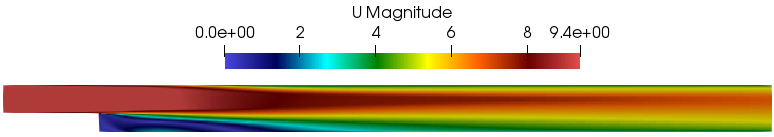
\includegraphics[width=\textwidth]{Images/valvel.png}
		\caption{Diagrama de contorno de la distribuci\'on de velocidad del sistema con part\'iculas de cobre de $70 [\mu m]$ - resultado obtenido al usar el modelo CFD-DEM desarrollado.}
	\end{subfigure}
	\caption{Comparaci\'on entre resultados del dise\~no experimental desarrollado por Fessler \& Eaton y los obtenidos a partir del modelo CFD-DEM desarrollado.}
	\label{resul1999}
\end{figure}

\noindent
\justify

Adicional al resultado mostrado en la Figura \ref{resul1999} $b)$, el modelo CFD-DEM desarrollado tambi\'en permite apreciar los resultados mostrados en la Figura \ref{valrel}.

\begin{figure}[h!]
	\centering
	\begin{subfigure}[b]{\textwidth}
		\centering
		
\includegraphics[width=\textwidth]{Images/valp.png}
		\caption{Diagrama de contorno de la variaci\'on de la fracci\'on de vac\'io en el volumen de control.}
	\end{subfigure}
	\hfill
	\begin{subfigure}[b]{\textwidth}
		\centering
		
\includegraphics[width=\textwidth]{Images/valk.png}
		\caption{Tendencia de distribuci\'on de las part\'iculas de cobre sobre el volumen de control.}
	\end{subfigure}
	\caption{Resultados obtenidos a partir del modelo CFD-DEM desarrollado.}
	\label{valrel}
\end{figure}

\noindent
\justify

La tendencia de distribuci\'on de las part\'iculas de cobre sobre el volumen de control se puede apreciar en la Figura \ref{valten}.

\begin{figure}[h!]
	\centering
	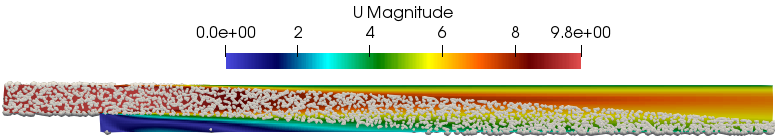
\includegraphics[width=1.1\textwidth]{Images/valpar.png}
	\caption{Distribuci\'on de las part\'iculas de cobre sobre la geometr\'ia.}
	\label{valten}
\end{figure}

\noindent
\justify

En la Figura \ref{valcompa} se puede apreciar la comparaci\'on directa en los perfiles de velocidad en diferentes puntos de inter\'es, contrastando los definidos por Fessler \& Eaton con respecto a los calculados por el modelo CFD-DEM desarrollado.

\begin{figure}[h!]
	\centering
	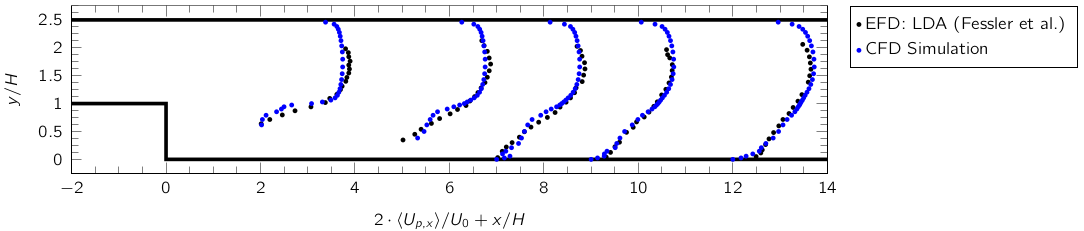
\includegraphics[width=1.1\textwidth]{Images/val.png}
	\caption{Comparaci\'on directa de los perfiles de velocidad experimentales con respecto al del modelo num\'erico desarrollado.}
	\label{valcompa}
\end{figure}

\noindent
\justify

En la Figura \ref{valcompa}, se aprecia una ligera variaci\'on entre los resultados experimentales con respecto a los obtenidos por el modelo num\'erico, reafirmando la exactitud de los resultados del modelo CFD-DEM; permitiendo as\'i validar el modelo desarrollado en el cap\'itulo \ref{CFD-DEM}.

\setcounter{secnumdepth}{0}
\begin{center}
	\section{Conclusiones}
\end{center}


\begin{enumerate}
	\item La presencia de v\'ortices y remolinos en la simulaci\'on CFD-DEM rectifica la decisi\'on de haber empleado un solucionador basado en \texttt{pimpleFoam}, el cual se adapt\'o para resolver el problema \textit{Euler - Lagrange} (E - L).
	\item Con base en los resultados obtenidos en la secci\'on \ref{CFDEM:resultados}, y analizados en la secci\'on \ref{CFDEM:analisis}, se reafirma la importancia de las simulaciones num\'ericas basadas en CFD-DEM para el dise\~no de maquinaria y equipos que busquen separar mezclas de sustancias s\'olidas y l\'iquidas. De la Figura \ref{CFDEM:part} se concluye que el panel de lamelas presenta zonas de salidas \textit{limpias} de material particulado y otras con una concentraci\'on menor a la inicialmente procesada. Futuras investigaciones podr\'ian emplear el modelo CFD-DEM desarrollado en el presente trabajo como base para el dise\~no de un nuevo sistema de sedimentaci\'on que emplee un \textit{reflujo} de las zonas con posibles impurezas para garantizar una completa separaci\'on de sustancias.
	\item Se implement\'o la metodolog\'ia del modelo CFD-DEM con base en herramientas de c\'odigo abierto; demostrando la viabilidad de estas herramientas en el desarrollo de nuevos productos y servicios de bajos costos de inversi\'on inicial y alto grado de innovaci\'on.
	\item De acuerdo al proceso de validaci\'on desarrollado en el cap\'itulo \ref{validacion}, se concluye que el modelo CFD-DEM desarrollado es preciso y puede ser empleado en diversas aplicaciones de flujo, bien sea laminar o turbulento, en donde part\'iculas s\'olidas interact\'uan con fluidos newtonianos en fase l\'iquida o gaseosa.
\end{enumerate}

\begin{center}
	\section{Recomendaciones}
\end{center}

\noindent
\justify

Al dise\~no final del sistema se le debe emplear un sistema de reflujo en la \'ultima lamela para garantizar una completa separaci\'on de la fase s\'olida y l\'iquida de la mezcla solvente extracto.

\noindent
\justify

Es recomendable construir un prototipo del sistema de sedimentaci\'on dise\~nado para ejecutar un dise\~no experimental con las variables descritas en el Cuadro \ref{exps}.

\begin{table}[h!]
	\centering
	\begin{tabular}{|c|c|}
		\hline
		\textbf{Variable} & \textbf{Rango} \\ \hline
		Temperatura & $[20 \, \degree C, 60 \, \degree C]$ \\ \hline
		Tiempo de separaci\'on $[h]$ & $[1, 4]$ \\ \hline
		Mezcla agua - etanol $[\% ]$ & $(0,25,50,75,100)$ \\ \hline
	\end{tabular}
	\caption{Dise\~no experimental sugerido.}
	\label{exps}
\end{table}

\noindent
\justify

Una vez seleccionada una especie vegetal de estudio, las variables de respuesta a analizar deber\'ian ser: rendimiento de extracci\'on (valor adimensional que contrasta la cantidad de material procesado con la cantidad de producto obtenido) y la composici\'on qu\'imica del extracto, obtenida mediante cromatograf\'ia l\'iquida (permite conocer la calidad del extracto).

\noindent
\justify

El software desarrollado, y documentado en el Anexo A, se puede complementar con m\'odulos de dibujo CAD a la geometr\'ia final (tanto 2D como 3D) e informes de ingenier\'ia autom\'atico en \LaTeX. Debido al hecho de haber sido desarrollado \'unicamente con lenguajes y herramientas de c\'odigo abierto, es posible crear un servicio de dise\~no web interactivo que resuelva simulaciones num\'ericas en la nube.
\setcounter{secnumdepth}{5}
\bibliography{library}
\begin{center}
	\section*{Anexo A: Software de dise\~no autom\'atico}
\end{center}

\noindent
\justify

Como complemento de la metodolog\'ia de dise\~no, se desarroll\'o un software de dise\~no autom\'atico (secci\'on \ref{software}) que, adicional al desarrollo de la metodolog\'ia de c\'alculo del dise\~no anal\'itico, incorpora un m\'odulo de discretizaci\'on de dominio (pudiendo desarrollar mallas estructuras y no estructuradas) y simulaci\'on autom\'atica a trav\'es de los m\'etodos CFD y CFD-DEM. A continuaci\'on, se puede apreciar la evidencia fotogr\'afica de los componentes del software desarrollado en Python - Jupyter.

\begin{figure}[h!]
	\centering
	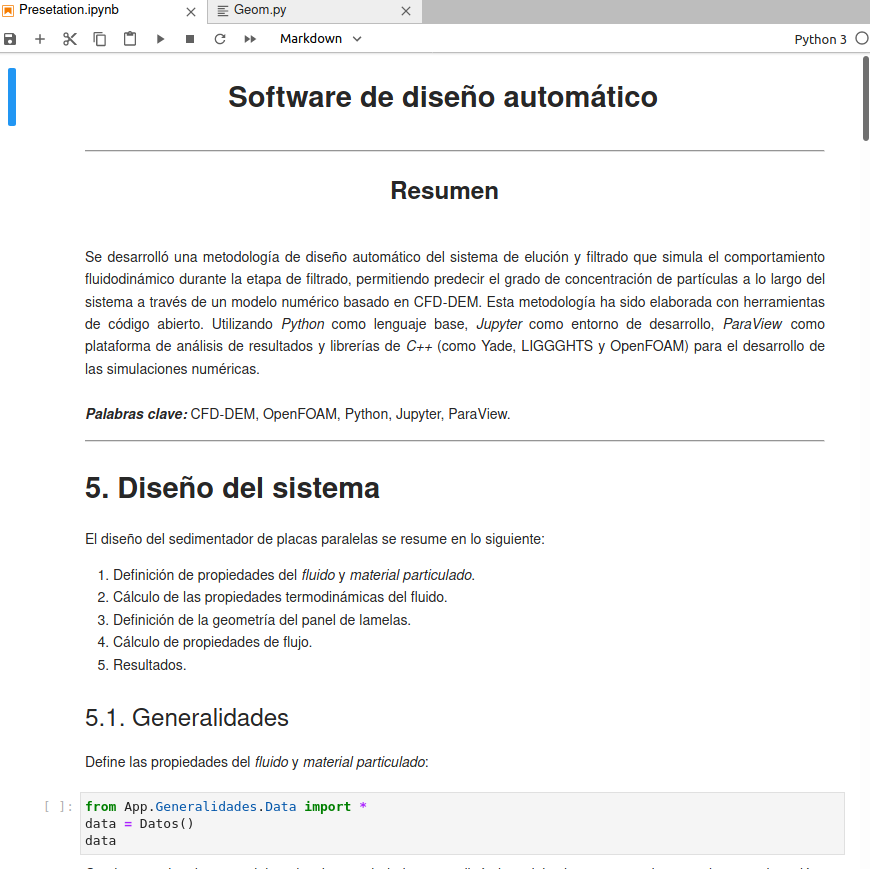
\includegraphics[width=\textwidth]{Images/Anexos/1.png}
	\caption{Inicio del software.}
	\label{inicioSoft}
\end{figure}

\noindent
\justify

Como se puede observar en la Figura \ref{inicioSoft}, el software se presenta en un formato de texto tipo pdf. Es como una especie de art\'iculo interactivo que permite ejecutar c\'odigo en vivo. El primer m\'odulo consiste en definir las condiciones de dise\~no de entrada; en t\'erminos de los datos del fluido y del material particulado. Una vez definidos los datos, se procede a calcular las propiedades termodin\'amicas.

\begin{figure}[h!]
	\centering
	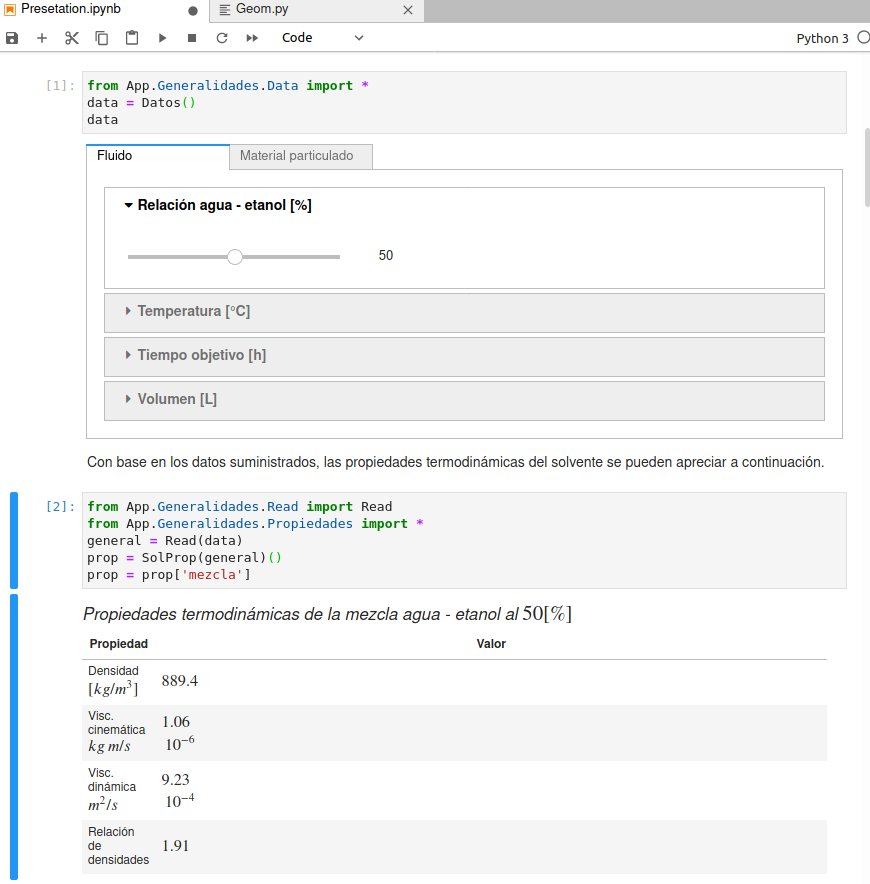
\includegraphics[width=\textwidth]{Images/Anexos/3.png}
	\caption{Datos y propiedades del solvente.}
	\label{propSoft}
\end{figure}

\newpage

\noindent
\justify

Una vez conocidas las propiedades del solvente, se procede a calcular la velocidad de asentamiento m\'axima de las part\'iculas.

\begin{figure}[h!]
	\centering
	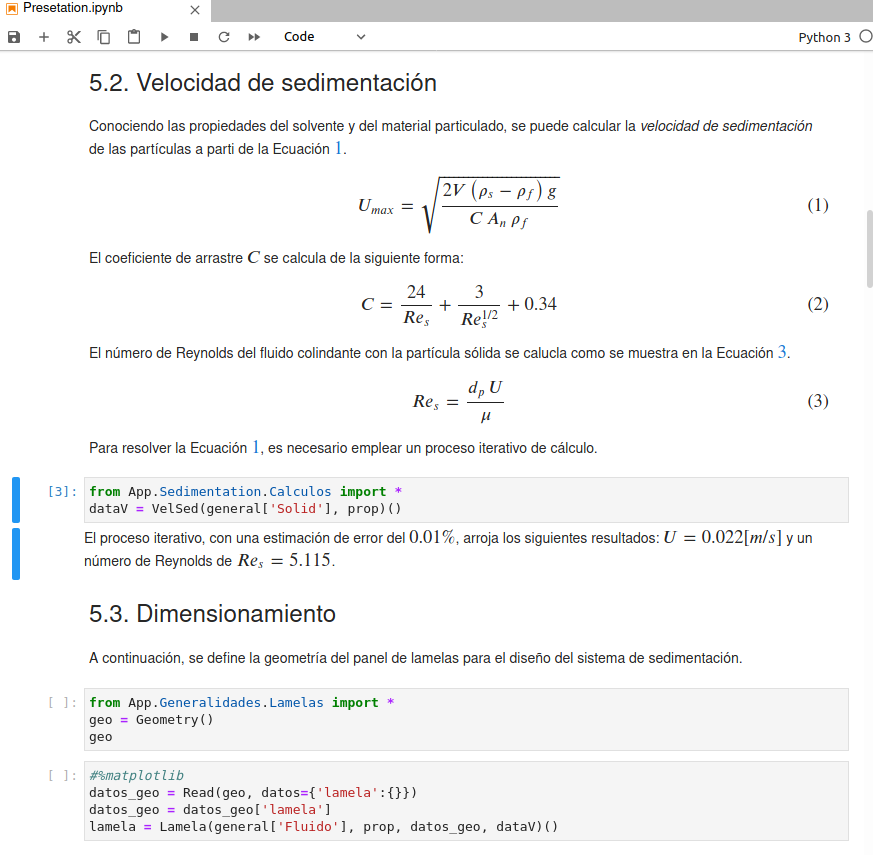
\includegraphics[width=\textwidth]{Images/Anexos/4.png}
	\caption{Velocidad de asentamiento m\'axima.}
	\label{velasSoft}
\end{figure}

\newpage

\noindent
\justify

Luego, se define una geometr\'ia inicial de dise\~no para el c\'alculo de las propiedades del fluido.

\begin{figure}[h!]
	\centering
	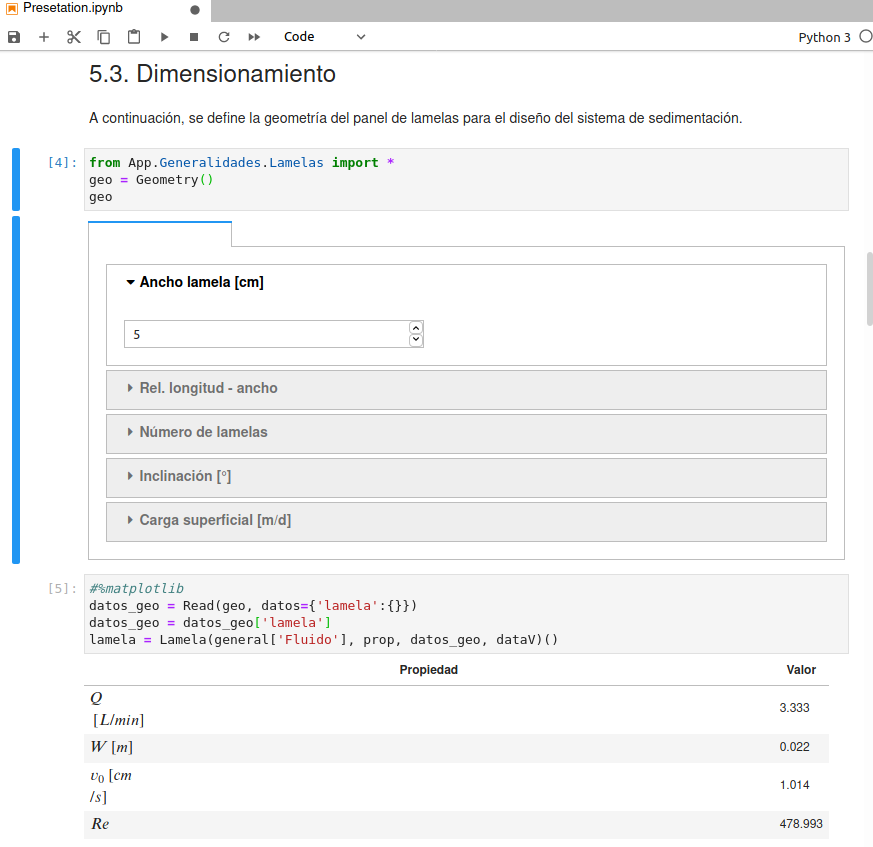
\includegraphics[width=\textwidth]{Images/Anexos/5.png}
	\caption{Geometr\'ia inicial.}
	\label{geoSoft}
\end{figure}

\newpage

\noindent
\justify

Una vez definida la geometr\'ia de estudio, con base en los criterios de dise\~no, se procede a discretizar el dominio especificando los datos referentes al mallado y al desarrollo de la geometr\'ia.

 \begin{figure}[h!]
	\centering
	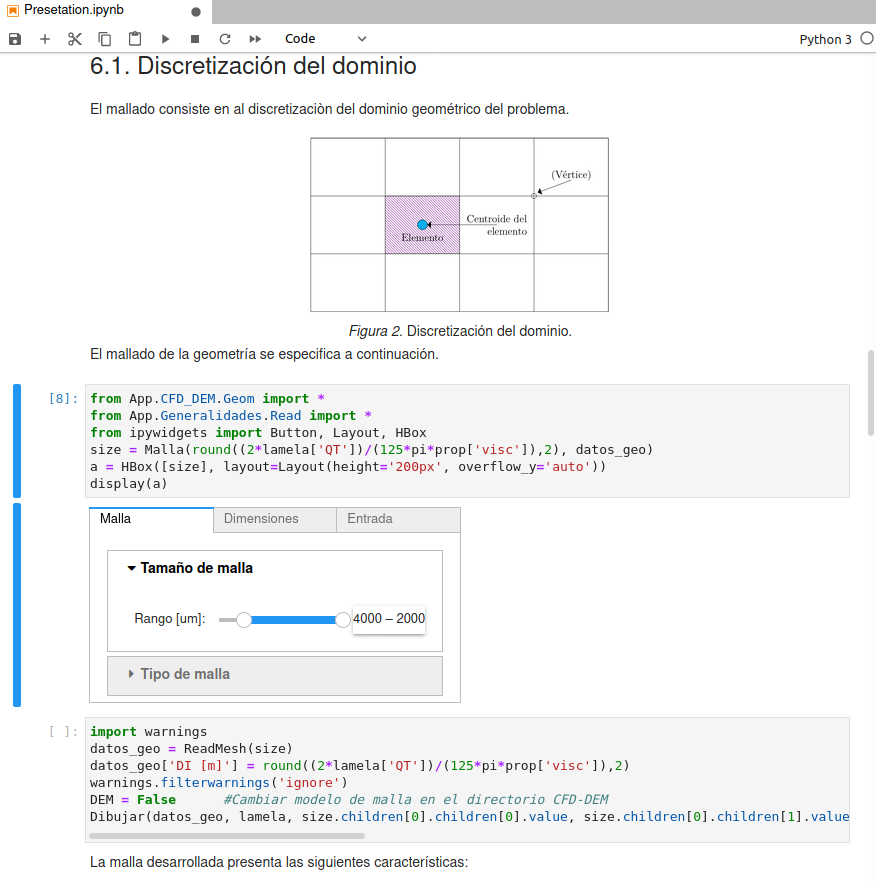
\includegraphics[width=\textwidth]{Images/Anexos/7.png}
	\caption{Datos del mallado de la geometr\'ia.}
	\label{dataMalla}
\end{figure}

\newpage

\noindent
\justify

Despu\'es, se procede a desarrollar la malla:

\begin{figure}[h!]
	\centering
	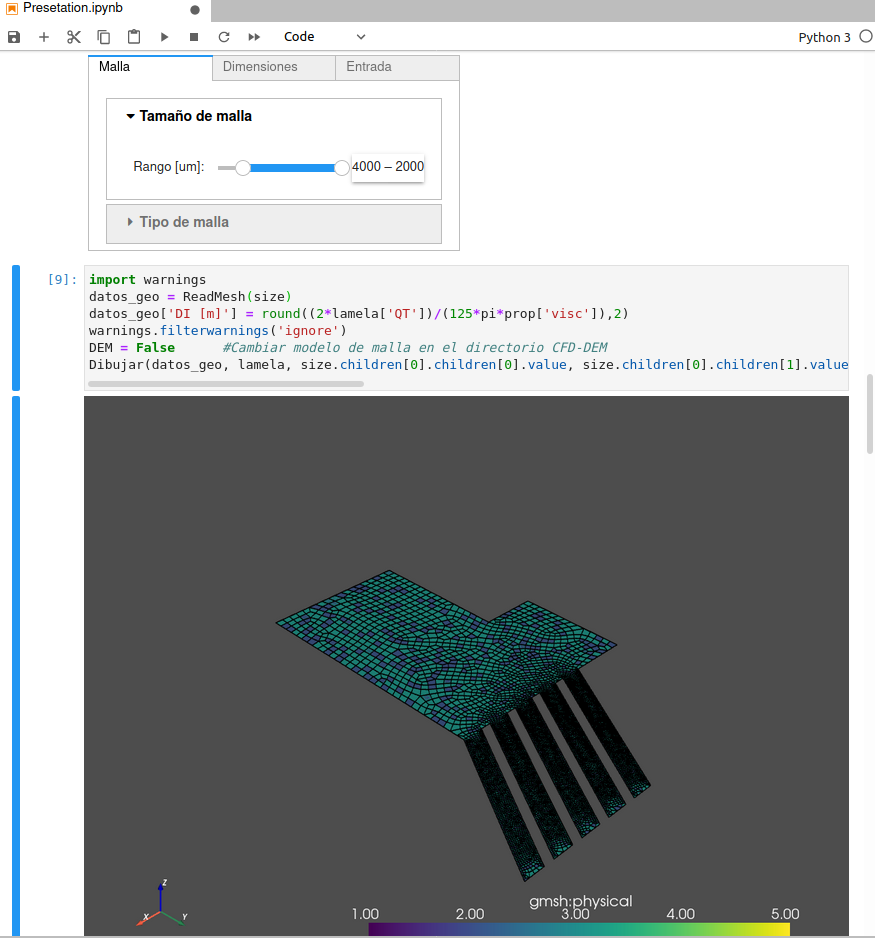
\includegraphics[width=\textwidth]{Images/Anexos/8.png}
	\caption{Mallado de la geometr\'ia.}
	\label{MallaSoft}
\end{figure}

\newpage

\noindent
\justify

Luego, se analizan las caracter\'isticas del mallado.

\begin{figure}[h!]
	\centering
	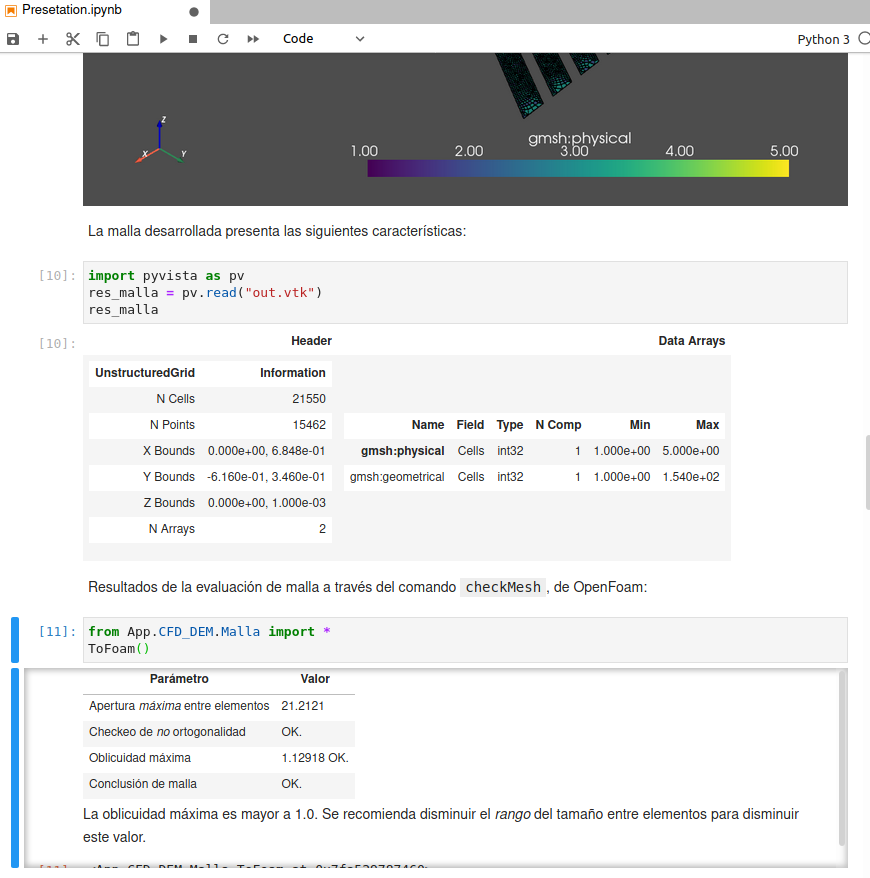
\includegraphics[width=\textwidth]{Images/Anexos/9.png}
	\caption{Caracter\'isticas del mallado.}
	\label{CarMallaSoft}
\end{figure}

\newpage

\noindent
\justify

En caso de que el mallado no sea el adecuado, es posible desarrollar cambios en los datos referentes a la geometr\'ia o al rango de tama\~nos de la malla.

\begin{figure}[h!]
	\centering
	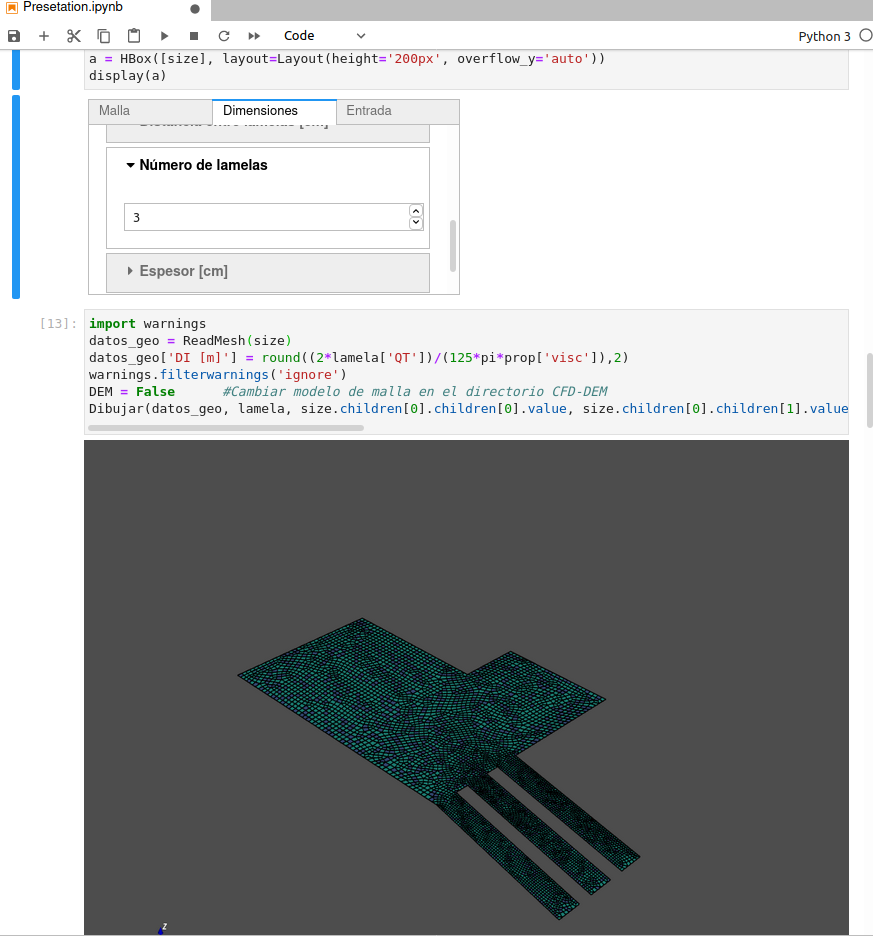
\includegraphics[width=\textwidth]{Images/Anexos/10.png}
	\caption{Cambios en el mallado.}
	\label{CamMallaSoft}
\end{figure}

\newpage

\noindent
\justify

Luego, se definen las condiciones de frontera:

\begin{figure}[h!]
	\centering
	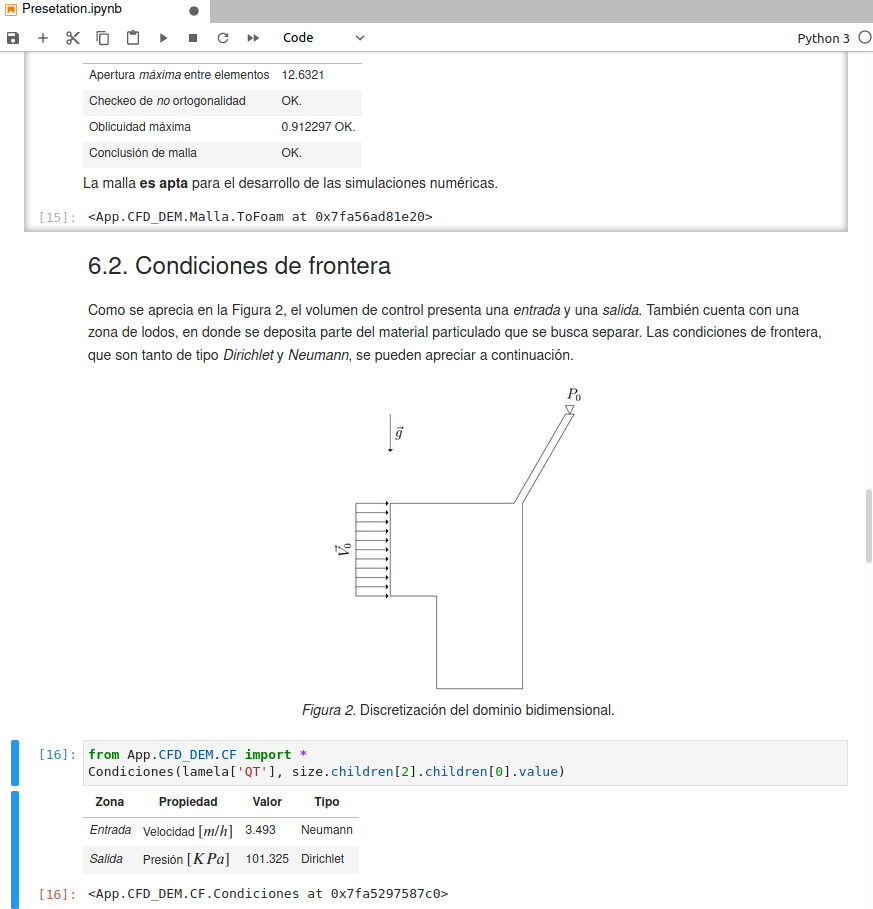
\includegraphics[width=\textwidth]{Images/Anexos/11.png}
	\caption{Cambios en el mallado.}
	\label{CamMallaSoft}
\end{figure}

\newpage

\noindent
\justify

Finalmente, se procede a realizar las simulaciones num\'ericas CFD y CFD-DEM.

\begin{figure}[h!]
	\centering
	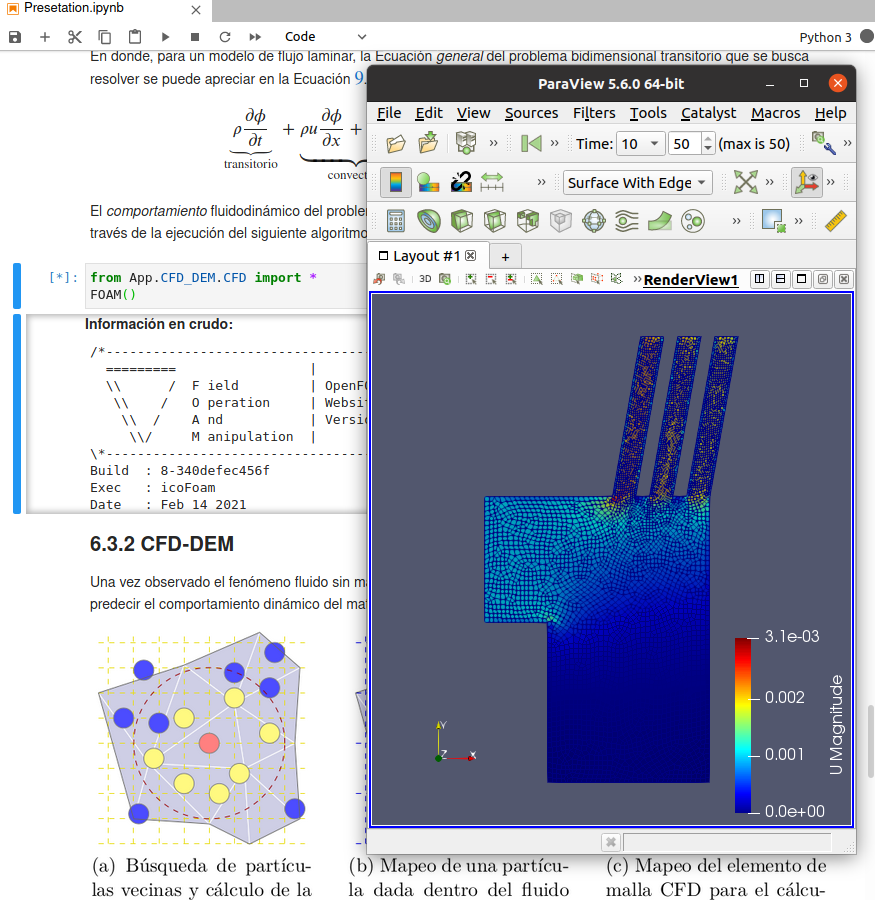
\includegraphics[width=\textwidth]{Images/Anexos/12.png}
	\caption{Cambios en el mallado.}
	\label{CamMallaSoft}
\end{figure}
\end{document}
